\documentclass {CSEThesis}
% Standard packages
\usepackage[T1]{fontenc}
\usepackage{amsmath}
\usepackage{graphicx}
\usepackage{epstopdf}
\usepackage{setspace}
\usepackage{multicol}
\usepackage{color}
\usepackage{booktabs}
\usepackage{longtable}
\usepackage{array}
\usepackage{tabularx}
\usepackage{multirow}
\usepackage{enumitem}
\usepackage{listings}
\lstdefinelanguage{JavaScript}{
  keywords={break,case,catch,continue,debugger,default,delete,do,else,
            finally,for,function,if,in,instanceof,new,return,switch,
            this,throw,try,typeof,var,void,while,with,
            const,let,class,export,import,async,await,of,from},
  morecomment=[l]{//},
  morecomment=[s]{/*}{*/},
  morestring=[b]',
  morestring=[b]",
  sensitive=true
}
\usepackage{float}
\usepackage[hidelinks]{hyperref}
\usepackage{url}
\usepackage{tikz}
\usetikzlibrary{arrows.meta, positioning, fit, backgrounds}
%===== page layout
% Define the side margins for a right-side page
%\insidemargin = 1.3in \outsidemargin = 0.9in
% Above margin is space above the header
% Below margin is space below footer
%\abovemargin = 1.5in \belowmargin = 0.05in


\btptitle = {Institutional Recruitment Portal: A Secure and Scalable MERN Stack Platform for Streamlining Project Hiring} % { and } are needed around your name
\name = {Tejas Kumar}          % and other feilds. don't remove.
\rollno = {2201MC42} \email = {2201mc42_tejas@iitp.ac.in} 
\guide = {Dr. Rahul Kumar Singh}
\coguide = {Dr. Mayank Agarwal}


\begin{document}

\begin{titlepage}
\begin{center}
{\large\sf  \textbf{\the\btptitle}}\\[12ex]
{\small{\textsl{ \textbf{A B. Tech Project Report Submitted \\
in Partial Fulfillment of the Requirements \\
for the Degree of
\\[3ex]\small \bf Bachelor of Technology}}}}\\[16ex] \emph{by} \\[2ex]
{\sf \sf \textbf{\the\name}\\
             (\the\rollno)}\\[1ex]
\emph{under the guidance of}\\[2ex]
{\sf \bf \the\guide} \\[1ex]
\emph{and}\\[1ex]
{\sf \bf \the\coguide} \\[5ex]

\vspace{0.5in}


\includegraphics[width=0.15\textwidth]{iitp_logo.eps}

\vspace{0.3in}

{\sl \bf{to the}} \\[1ex]

{\small\bf DEPARTMENT OF MATHEMATICS}  \\[1ex]
{\small \bf{INDIAN INSTITUTE OF TECHNOLOGY PATNA \\ PATNA -- 800013, BIHAR}}
%\\[2ex]
%
%  {\color{red} \hrule height 0.5ex}
% \vskip 1ex
% May \the\year
\end{center}
\end{titlepage}
\cleardoublepage
\raggedbottom
\doublespacing
\pagenumbering{roman}
\chapter*{\centering \underline{CERTIFICATE}}
\vskip 2ex \emph{\quad This is to certify that the work contained
in this thesis entitled ``\textbf{\the\btptitle}'' is a bonafide
work of \textbf{\the\name} (\textbf{Roll No. \the\rollno}),
carried out in the Department of Computer Science and Engineering,
Indian Institute of Technology Patna under my supervision and that
it has not been submitted elsewhere for a degree.} \vskip 10ex

\noindent
\begin{minipage}[t]{0.35\textwidth}
  \vspace{1cm}
  \textbf{\the\name}\\
  Roll No. \the\rollno
\end{minipage}
\hfill
\begin{minipage}[t]{0.55\textwidth}
  \raggedleft
  \vspace{1cm}
  Supervisor: \textbf{\the\guide}\\
  Department of Mathematics,\\
  Indian Institute of Technology Patna.\\
  \vspace{1cm}
  Co-supervisor: \textbf{\the\coguide}\\
  Department of Computer Science \& Engineering,\\
  Indian Institute of Technology Patna.
\end{minipage}

\vskip 4ex
\noindent May, \the\year\\
Patna.

\cleardoublepage
\chapter*{\centering Acknowledgements}

\quad I would like to express my sincere gratitude to everyone who supported and guided me throughout the development of this project and the preparation of this thesis.

First and foremost, I am deeply grateful to my supervisor, \textbf{Dr.\ Rahul Kumar Singh}, and my co-supervisor, \textbf{Dr.\ Mayank Agarwal}, for their invaluable guidance, continuous encouragement, and insightful feedback at every stage of this project. Their expertise and constructive suggestions were instrumental in shaping the architecture and quality of the Institutional Recruitment Portal.

I extend my gratitude to the \textbf{Department of Mathematics}, IIT Patna, for providing access to the computational resources required for development and testing.

I am also thankful to my fellow batch-mates and friends whose peer reviews, technical discussions, and moral support kept me motivated throughout this journey.

Finally, I owe a heartfelt debt of gratitude to my \textbf{family} for their unwavering support, patience, and encouragement throughout my undergraduate years and the completion of this project.

\vspace{1cm}
\begin{flushright}
\textbf{Tejas Kumar}\\
Roll No.\ 2201MC42\\
\end{flushright}

\cleardoublepage
\newpage
\chapter*{\centering Abstract}

Managing recruitment for institutional projects in educational institutions often involves manual handling of applications through emails or paper documents, leading to fragmented applicant data, difficulty in managing multiple projects, and limited transparency. The Institutional Recruitment Portal is a secure, web-based platform designed to streamline and digitize the end-to-end recruitment workflow for project-specific hiring. The system provides a unified environment for Administrators, Professors, and Applicants.

The platform enables professors to create and manage project listings, set deadlines, and define required documents. Applicants can securely register, apply for specific projects, and upload necessary credentials such as ID proofs, academic documents, and payment receipts. The system implements a structured local filesystem storage architecture, replacing traditional cloud dependencies for better institutional control and faster document management. Security is ensured through JSON Web Token (JWT) authentication, Role-Based Access Control (RBAC), and bcrypt password hashing.

The system is built on the MERN stack (MongoDB, Express.js, React, Node.js), containerized with Docker, and served through Nginx. Key administrative features include professor management, project moderation, and comprehensive application tracking. The portal also supports bulk document downloads as ZIP archives and application data export in CSV format, facilitating efficient post-application processing.

Evaluation demonstrates that the Institutional Recruitment Portal significantly reduces manual overhead, improves data accessibility for professors, and provides a professional, streamlined experience for applicants, thereby establishing a robust digital infrastructure for institutional project management.

\cleardoublepage
\tableofcontents
\cleardoublepage
\addcontentsline{toc}{chapter}{List of Figures}
\listoffigures
\cleardoublepage
\addcontentsline{toc}{chapter}{List of Tables}
\listoftables
\cleardoublepage
\pagenumbering{arabic}
\def\headrulehook{\color{black}}      % Color the header rule

%========== Chapters
\typeout{}
\chapter{Introduction}
\pagenumbering{arabic}\hspace{3mm}

\section{Background and Motivation}

Academic institutions like IIT Patna frequently undertake research and consultancy projects that require the recruitment of project staff, such as Junior Research Fellows (JRF), Senior Research Fellows (SRF), and project assistants. Traditionally, this recruitment process has been handled through manual or semi-automated methods. Typically, a project advertisement is released, and candidates are asked to send their applications, including resumes and supporting documents, via email or physical post to the concerned principal investigator (Professor).

This traditional approach leads to several inefficiencies. Professors often receive hundreds of emails, making it difficult to track and organize applications for multiple projects simultaneously. There is no centralized system to verify if a candidate has submitted all required documents, and managing the status of each application (e.g., shortlisted, rejected) is a tedious manual task. Furthermore, the lack of a standardized application format makes it challenging to compare candidates efficiently. A purpose-built, secure, and scalable recruitment portal tailored to the institutional context is therefore both timely and necessary.

To address these challenges, the \textbf{Institutional Recruitment Portal} is proposed and developed. This is a MERN-stack-based web application designed to digitize the entire recruitment workflow, from project advertisement to candidate selection. The system leverages role-based access control to ensure that only authorized personnel can manage projects and view sensitive candidate information.

\section{Problem Statement}

The institutional recruitment process currently faces the following operational challenges, which this portal is designed to address:

\begin{enumerate}
  \item \textbf{Fragmentation of Application Data.} Applications and supporting documents are often scattered across multiple email inboxes or physical folders, making centralized tracking impossible.
  
  \item \textbf{Manual Document Verification.} There is no automated way to ensure that applicants have uploaded all mandatory documents (e.g., GATE score, mark sheets) before their application is considered.
  
  \item \textbf{Difficulty in Managing Multiple Projects.} Professors handling multiple research projects simultaneously struggle to separate and manage applicant pools for each project efficiently.
  
  \item \textbf{Lack of a Standardized Application Flow.} Applicants often submit information in varying formats, making it difficult for professors to extract and compare key data points.
  
  \item \textbf{Security and Privacy Concerns.} Handling sensitive personal documents (like ID proofs) via email is less secure than using a dedicated platform with encrypted storage and access control.
  
  \item \textbf{Lack of Institutional Oversight.} The administration has no real-time visibility into the recruitment activities across different departments and projects.
\end{enumerate}

\section{Objectives}

The primary objective of this project is to design, implement, and evaluate a comprehensive web-based recruitment management system. The specific objectives are:

\begin{enumerate}
  \item Develop a centralized platform for project advertisements and application submissions.
  
  \item Implement a secure multi-portal system for Students (Applicants), Professors, and Administrators.
  
  \item Design a structured local filesystem storage system for managing large volumes of uploaded documents.
  
  \item Enable professors to manage their own projects, view applications in real-time, and update application statuses.
  
  \item Provide data export features, including bulk ZIP downloads of documents and CSV exports of application summaries.
  
  \item Ensure high security through JWT-based authentication and Role-Based Access Control (RBAC).
  
  \item Build a responsive and premium user interface to enhance the user experience for all stakeholders.
\end{enumerate}

\section{Scope of the Project}

\subsection{In Scope}

The following capabilities are within the scope of the Institutional Recruitment Portal:

\begin{itemize}
  \item User registration and authentication (Student, Professor, Admin).
  \item Project creation, editing, and deletion by Professors.
  \item Application submission with mandatory document uploads.
  \item Local filesystem storage structured by project code and applicant name.
  \item Role-based dashboard for all three user roles.
  \item Status management (Pending, Qualified, Rejected) for applications.
  \item CSV export of application data for further processing.
  \item Bulk ZIP download of all documents associated with a project.
  \item Containerized deployment using Docker and Nginx.
\end{itemize}

\subsection{Out of Scope}

The following are explicitly excluded from the current version:

\begin{itemize}
  \item Online interview scheduling or video conferencing integration.
  \item Automated resume screening using AI/ML.
  \item Integration with external job boards (e.g., LinkedIn).
  \item Payment gateway integration for application fees.
  \item Real-time chat between professors and applicants.
\end{itemize}

\section{Key Contributions}

The principal contributions of this project are:

\begin{enumerate}
  \item A fully functional, production-ready MERN stack application that digitizes the entire institutional recruitment lifecycle.
  
  \item A robust and structured file management system that handles large-scale document uploads without relying on expensive cloud storage providers.
  
  \item A secure, role-aware architecture that ensures the privacy of applicant data and the integrity of the recruitment process.
  
  \item A data-driven approach to recruitment, providing tools for easy export and analysis of applicant pools.
\end{enumerate}

\section{Organisation of The Report}

The remainder of this report is organized as follows.
In Chapter~2, existing recruitment platforms and the technical foundations of the MERN stack are reviewed.
In Chapter~3, the system design and architecture are presented, including the three-portal structure and the database schema.
In Chapter~4, the implementation details, including local storage logic and security measures, are discussed.
Finally, Chapter~5 concludes the report and suggests future improvements.
\cleardoublepage
\typeout{}
\chapter{Literature Review}

\section{Recruitment Management Systems}

Recruitment Management Systems (RMS), also known as Applicant Tracking Systems (ATS), have become essential tools for modern human resource management. Traditionally, these systems were designed for large corporations to handle high volumes of resumes. However, there is an increasing need for lightweight, specialized systems tailored for academic and research institutions.

According to research by Smith et al. (2020), automated recruitment systems can reduce the time-to-hire by up to 40\% by automating repetitive tasks such as document collection and status tracking. In the institutional context, where recruitment is often decentralized across various research projects, a centralized RMS provides a single source of truth for both administration and professors.

\section{MERN Stack in Web Development}

The MERN stack (MongoDB, Express.js, React, Node.js) has emerged as a leading architecture for building scalable web applications. The stack uses JavaScript across the entire development lifecycle, reducing context-switching for developers and allowing for a more unified codebase.

MongoDB, a NoSQL document database, is particularly suited for recruitment systems where application forms might vary between projects. As noted by Johnson (2021), the flexible schema of MongoDB allows for easy extension of data models without the downtime associated with traditional relational database migrations.

\section{Security in Web-Based Recruitment}

Security and privacy are paramount when handling applicant data, which often includes sensitive personal identifiers and academic credentials. The OWASP Top Ten (2021) provides a framework for addressing common web vulnerabilities.

Key security measures for recruitment portals include:
\begin{itemize}
  \item \textbf{JWT Authentication:} Stateless authentication that prevents session-based vulnerabilities.
  \item \textbf{Role-Based Access Control (RBAC):} Ensuring that professors can only see applications for their own projects and that students cannot access other candidates' data.
  \item \textbf{Data Sanitization:} Preventing SQL/NoSQL injection and Cross-Site Scripting (XSS) through rigorous input validation.
\end{itemize}

\section{Local vs. Cloud Storage}

While cloud storage providers like AWS S3 or Cloudinary offer convenience, institutional servers often prefer local filesystem storage for cost-effectiveness and data sovereignty. Implementing a structured local storage system requires careful directory management and collision-resistance logic, as implemented in this project using Multer.

\section{Summary}

The literature suggests that while general-purpose recruitment systems exist, there is a clear gap for institutional portals that support project-specific hierarchies and local document management. The Institutional Recruitment Portal fills this gap by combining the modern MERN stack with a secure, role-aware architecture optimized for institutional servers.

\cleardoublepage
\typeout{}
\chapter{System Design and Architecture}

\section{System Overview}

The Institutional Recruitment Portal is built using a modern three-tier architecture, designed for scalability, security, and maintainability. The system consists of a presentation layer (React SPA), a business logic layer (Node.js/Express API), and a data layer (MongoDB). The entire system is containerized using Docker, with Nginx serving as a reverse proxy and static file server.

Figure~\ref{fig:architecture} illustrates the high-level architecture. The frontend communicates with the backend via RESTful APIs using JSON for data exchange. The backend handles authentication, authorization, file processing, and database interactions.

\begin{figure}[htbp]
  \centering
  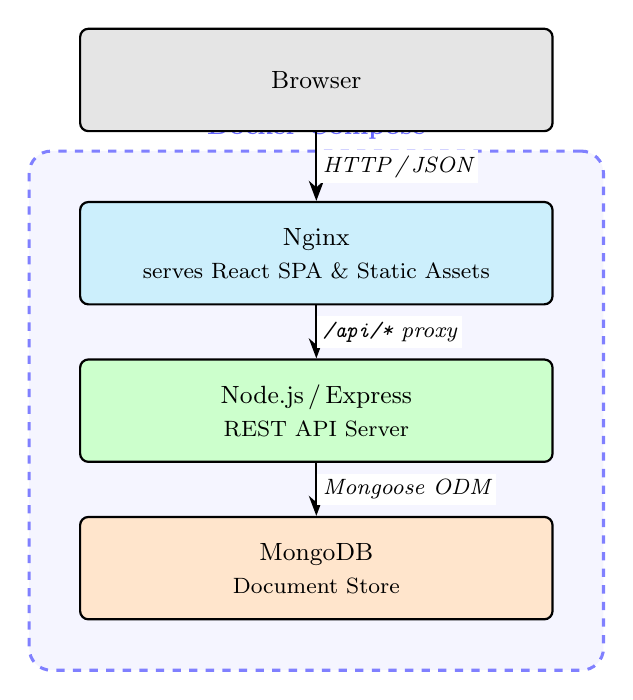
\begin{tikzpicture}[
    box/.style  = {draw, rectangle, rounded corners=3pt, thick,
                   minimum width=6cm, minimum height=1.3cm,
                   align=center, font=\small},
    arr/.style  = {-{Stealth[scale=1.1]}, thick},
    note/.style = {font=\footnotesize\itshape, fill=white, inner sep=2pt}
  ]
    \node[box, fill=gray!20]   (browser) at (0, 7.8) {Browser};
    \node[box, fill=cyan!20]   (nginx)   at (0, 5.6)
          {Nginx\\[1pt]{\footnotesize serves React SPA \& Static Assets}};
    \node[box, fill=green!20]  (express) at (0, 3.6)
          {Node.js\,/\,Express\\[1pt]{\footnotesize REST API Server}};
    \node[box, fill=orange!20] (mongo)   at (0, 1.6)
          {MongoDB\\[1pt]{\footnotesize Document Store}};

    \draw[arr] (browser) -- node[note,right]{HTTP\,/\,JSON}         (nginx);
    \draw[arr] (nginx)   -- node[note,right]{\texttt{/api/*} proxy}  (express);
    \draw[arr] (express) -- node[note,right]{Mongoose ODM}           (mongo);

    \begin{scope}[on background layer]
      \node[draw=blue!50, dashed, line width=1.1pt, rounded corners=8pt,
            fill=blue!4, inner xsep=18pt, inner ysep=18pt,
            fit=(nginx)(express)(mongo),
            label={[blue!60, font=\small\bfseries]above:Docker Compose}] {};
    \end{scope}
  \end{tikzpicture}
  \caption{Three-tier architecture of the Recruitment Portal.}
  \label{fig:architecture}
\end{figure}

\section{User Roles and Access Control}

The system implements Role-Based Access Control (RBAC)~\cite{Sandhu1996} with three distinct portals:

\begin{enumerate}
  \item \textbf{Student (Applicant) Portal:} Allows candidates to register, browse project listings, and submit applications. Applicants can track the status of their submissions and manage their profiles.
  
  \item \textbf{Professor Portal:} Provides tools for professors to create and manage project advertisements. Professors can view detailed applicant profiles, download uploaded documents, and update the recruitment status for each applicant.
  
  \item \textbf{Admin Portal:} Offers high-level oversight, including professor management (approving/blocking accounts), project moderation, and global application tracking.
\end{enumerate}

Table~\ref{tab:roles} summarizes the permissions and primary capabilities for each role.

\begin{table}[H]
  \centering
  \caption{User roles and primary capabilities in the Recruitment Portal.}
  \label{tab:roles}
  \begin{tabularx}{\textwidth}{lX}
    \hline
    \textbf{Role} & \textbf{Primary Capabilities} \\
    \hline
    Administrator & Full system access; Professor account approval; Project moderation; Global application tracking; System configuration. \\
    Professor     & Create and manage projects; View applicant profiles; Download application ZIPs; Export CSV data; Update application status. \\
    Student       & Register and manage profile; Browse active projects; Submit project applications; Upload documents; Track status. \\
    \hline
  \end{tabularx}
\end{table}

\section{Database Design}

MongoDB is used for its flexible schema, which is ideal for handling varying project requirements and applicant data. The primary collections are:

\begin{itemize}
  \item \textbf{Users:} Stores authentication credentials, roles, and basic profile information.
  \item \textbf{Professors:} Extends the User model with department and designation details.
  \item \textbf{Projects:} Contains project codes, titles, descriptions, deadlines, and the ID of the owning professor.
  \item \textbf{Applications:} Links students to projects and professors. It stores the applicant's name, submitted form data, application status, and paths to uploaded documents.
\end{itemize}

Table~\ref{tab:collections} provides a summary of the MongoDB collections and their purposes.

\begin{table}[H]
  \centering
  \caption{Summary of MongoDB collections in the Recruitment Portal.}
  \label{tab:collections}
  \begin{tabularx}{\textwidth}{llX}
    \hline
    \textbf{Collection} & \textbf{Est.\ Docs} & \textbf{Description} \\
    \hline
    Users               & Per system user     & Authentication and role-based access data. \\
    Professors          & Per faculty         & Extended profile for faculty members. \\
    Projects            & Per listing         & Project details, requirements, and deadlines. \\
    Applications        & Per submission      & Student data linked to specific projects. \\
    \hline
  \end{tabularx}
\end{table}

\section{File Storage Architecture}

A key architectural decision was the implementation of a structured local filesystem storage system using Multer. Instead of relying on external cloud storage, the system organizes files in a hierarchical directory structure on the server:

\begin{lstlisting}[float=htbp, language=bash, caption={Uploads directory structure.}]
uploads/
|-- <projectCode>/
|   |-- <applicantName>_<serialNumber>/
|   |   |-- <applicantName>_<serial>_photo.jpg
|   |   |-- <applicantName>_<serial>_resume.pdf
|   |   `-- <applicantName>_<serial>_id_proof.pdf
\end{lstlisting}

This structure ensures that files are easily locatable, collision-resistant, and can be efficiently zipped for bulk download.

\section{Security Architecture}

The system follows a security-first approach:

\begin{itemize}
  \item \textbf{Authentication:} Stateless authentication using JWT.
  \item \textbf{Password Hashing:} Secure hashing using bcrypt.
  \item \textbf{Input Validation:} All API endpoints use \texttt{express-validator} for strict schema enforcement.
  \item \textbf{CORS:} Restricts API access to authorized origins.
  \item \textbf{Static Serving:} Nginx serves the frontend and handles the reverse proxying to the backend, hiding the internal API structure.
\end{itemize}

\section{API Design}

The backend exposes a RESTful API following standard HTTP conventions~\cite{Fielding2000}. Table~\ref{tab:api} lists the major route groups.

\begin{table}[H]
  \centering
  \caption{Principal REST API route groups in the Recruitment Portal.}
  \label{tab:api}
  \begin{tabularx}{\textwidth}{llX}
    \hline
    \textbf{Prefix} & \textbf{Method(s)} & \textbf{Description} \\
    \hline
    \texttt{/api/auth}         & POST           & Login, registration, password management. \\
    \texttt{/api/users}        & GET, PUT       & User profile and account management. \\
    \texttt{/api/professors}   & GET, POST, PUT & Professor onboarding and moderation. \\
    \texttt{/api/projects}     & GET, POST, DELETE & Project listing lifecycle. \\
    \texttt{/api/applications} & GET, POST, PUT & Application submission and status tracking. \\
    \texttt{/api/admin}        & GET, PUT       & System-wide oversight and dashboard data. \\
    \hline
  \end{tabularx}
\end{table}

\section{User Interface Design}

The Recruitment Portal features a clean, professional interface tailored for each user role. The Student dashboard provides a clear overview of available projects, while the Admin dashboard focuses on system-wide statistics and management.

\begin{figure}[H]
  \centering
  \setlength{\fboxsep}{0pt}
  \setlength{\fboxrule}{0.2pt}
  \fbox{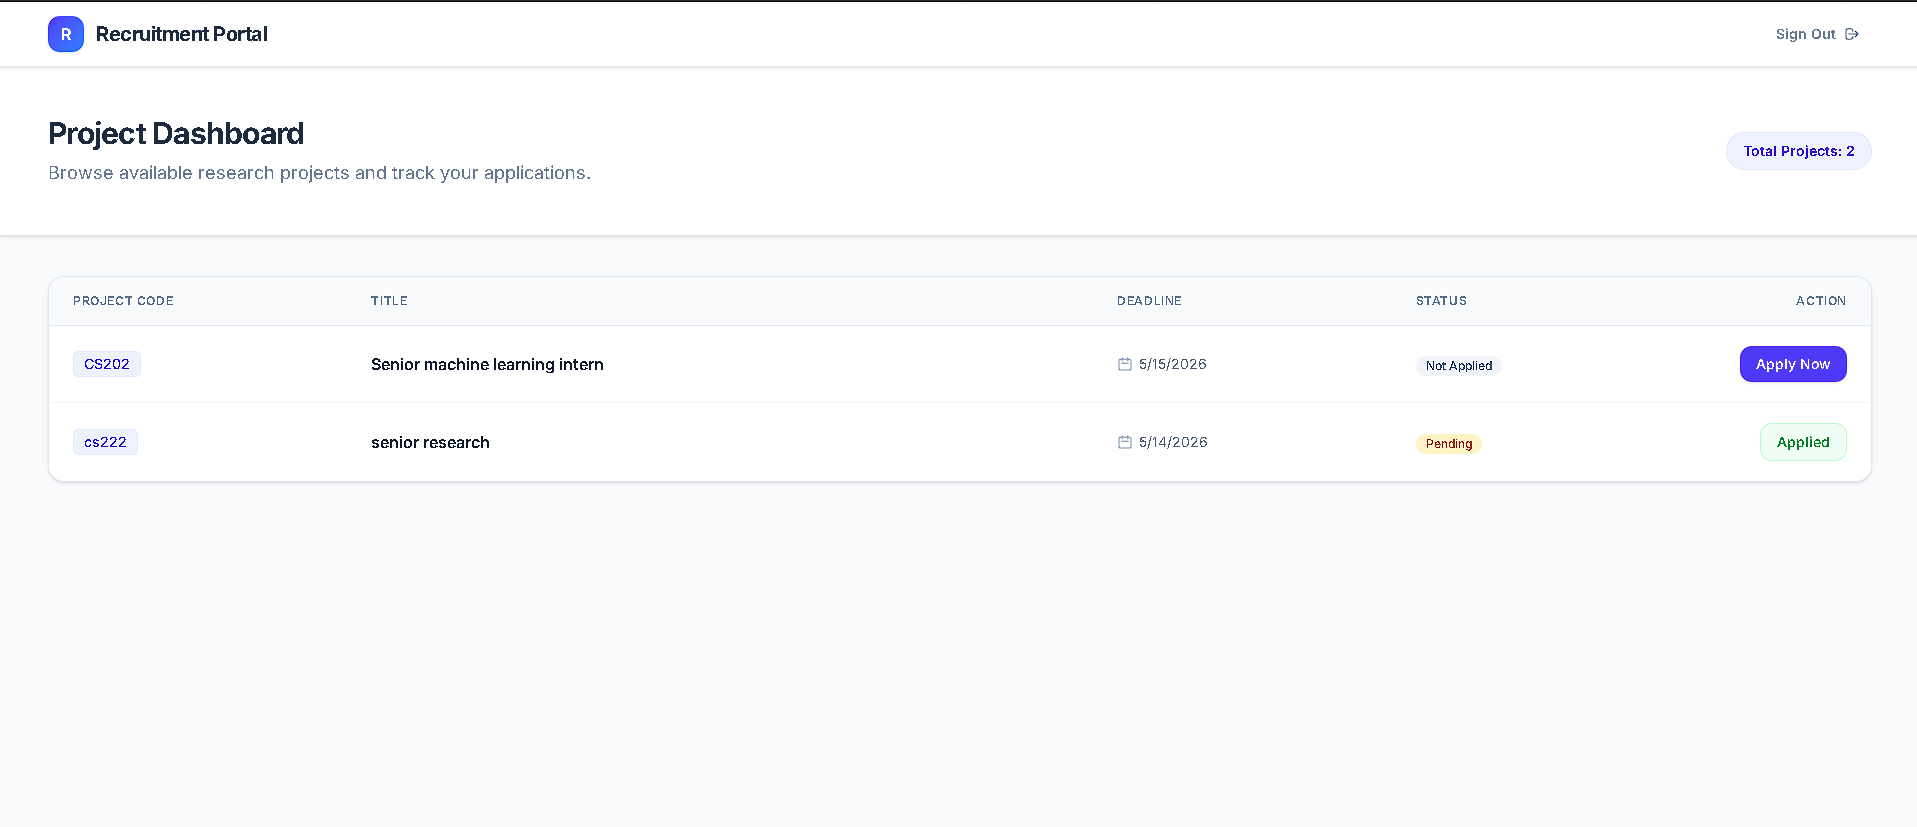
\includegraphics[width=0.85\textwidth]{figures/student_dashboard.png}}
  \caption{Student dashboard showing active project listings and application status.}
  \label{fig:student_dash}
\end{figure}

\begin{figure}[H]
  \centering
  \setlength{\fboxsep}{0pt}
  \setlength{\fboxrule}{0.2pt}
  \fbox{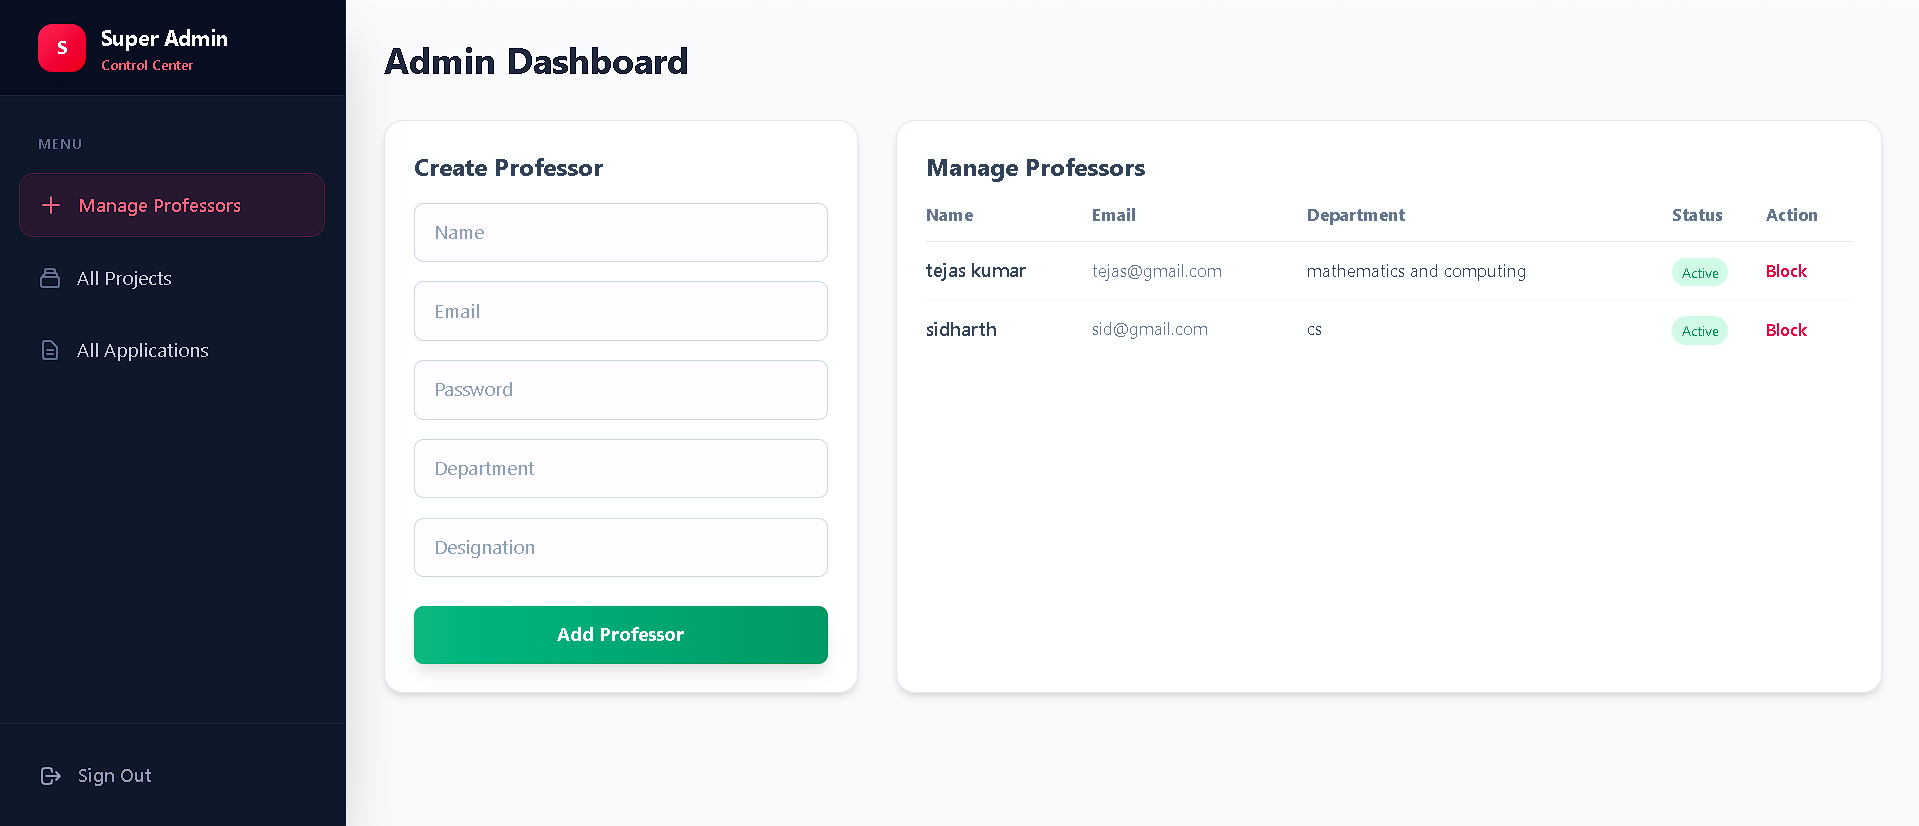
\includegraphics[width=0.85\textwidth]{figures/admin_dashboard.png}}
  \caption{Admin dashboard providing an overview of total professors, projects, and applications.}
  \label{fig:admin_dash}
\end{figure}

\begin{figure}[H]
  \centering
  \setlength{\fboxsep}{0pt}
  \setlength{\fboxrule}{0.2pt}
  \fbox{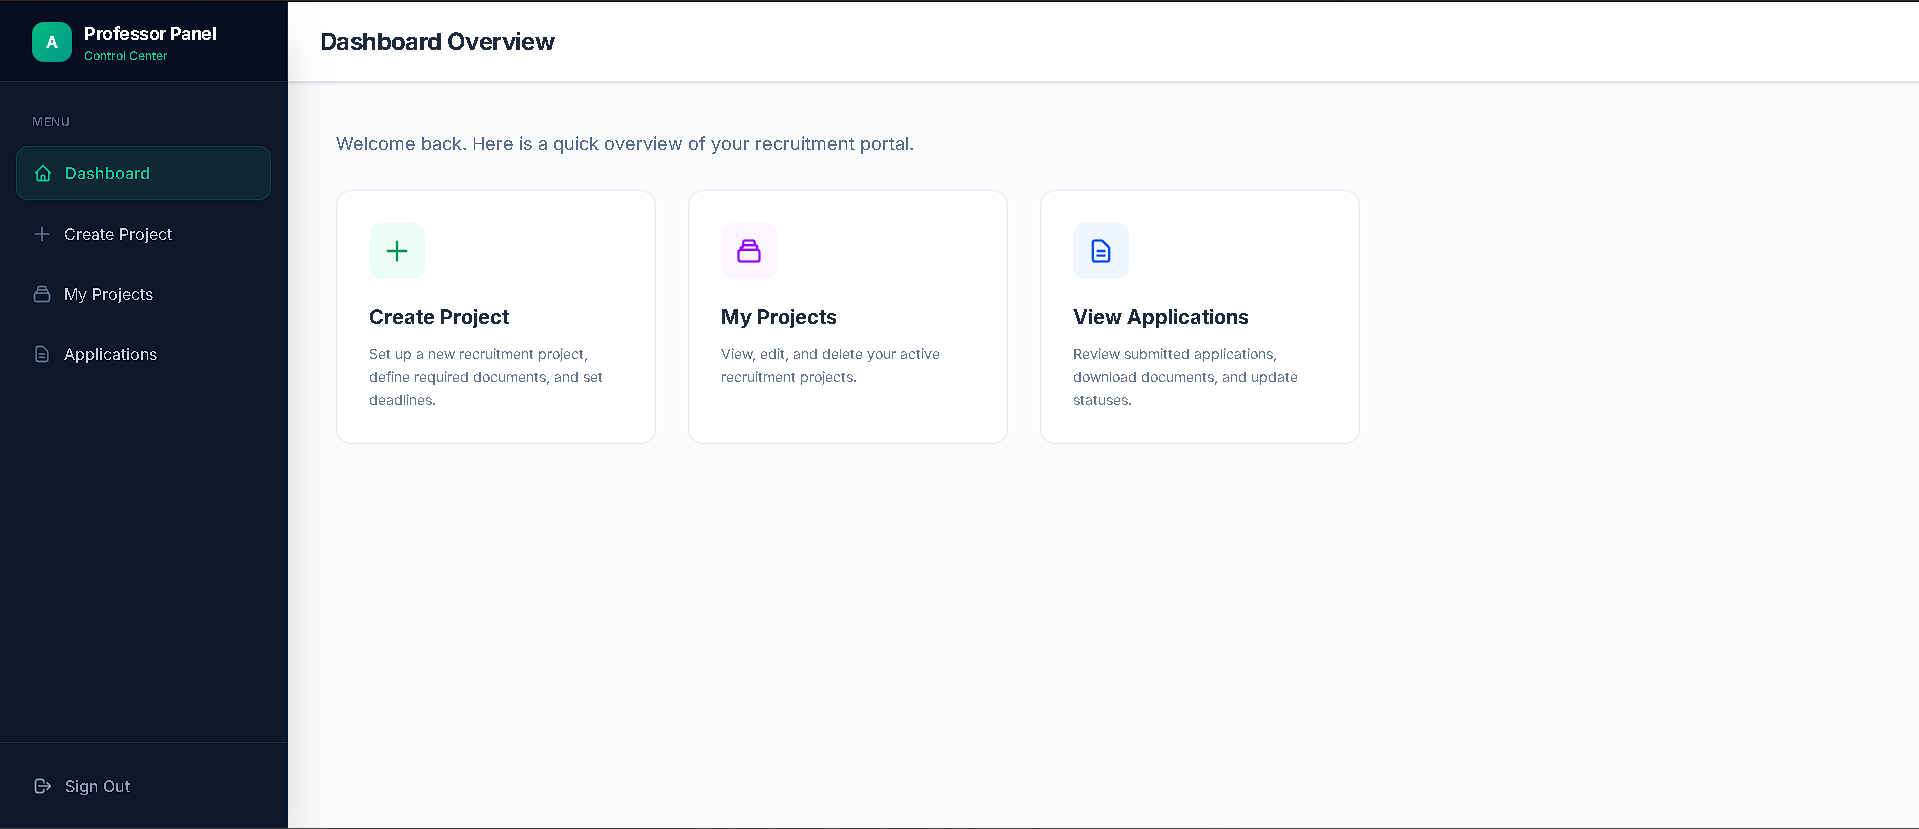
\includegraphics[width=0.85\textwidth]{figures/professor_dashboard.png}}
  \caption{Professor dashboard providing a summary of managed projects and application statistics.}
  \label{fig:prof_dash}
\end{figure}

\cleardoublepage
\typeout{}
\chapter{Implementation}

This chapter discusses the technical implementation of the Recruitment Portal, covering the development environment, technology stack, and core logic for file management and security.

\section{Technology Stack}

The system is built using the MERN stack. Table \ref{tab:stack} summarizes the primary technologies used.

\begin{table}[htbp]
  \centering
  \caption{Recruitment Portal Technology Stack.}
  \label{tab:stack}
  \begin{tabularx}{\textwidth}{llX}
    \hline
    \textbf{Component}    & \textbf{Technology}      & \textbf{Rationale} \\
    \hline
    Backend               & Node.js / Express        & High-performance, event-driven API handling. \\
    Frontend              & React / Vite             & Fast, component-based UI development. \\
    Database              & MongoDB / Mongoose       & Flexible schema for project-specific application forms. \\
    Styling               & Tailwind CSS             & Rapid development of premium, responsive UI~\cite{Tailwind2024}. \\
    Auth                  & JWT / bcrypt             & Secure, stateless authentication~\cite{RFC7519}. \\
    File Uploads          & Multer                   & Local disk storage for institutional control. \\
    ZIP Generation        & Archiver                 & Efficient bulk document packaging. \\
    Containerization      & Docker                   & Ensures environment consistency~\cite{Docker2024}. \\
    \hline
  \end{tabularx}
\end{table}

\section{Backend Implementation}

The backend is structured into routes, controllers, and models. A central \texttt{index.js} entry point initializes the Express server and connects to MongoDB.

\subsection{Local File Storage Logic}

A custom Multer disk storage engine was implemented to organize uploads by project and applicant. The `resolveProject` middleware runs before the upload to determine the target directory based on the project code.

\begin{lstlisting}[language=JavaScript, caption={Multer disk storage configuration.}]
const storage = multer.diskStorage({
  destination: function (req, file, cb) {
    const projectCode = req.resolvedProjectCode || "unresolved";
    const applicantFolder = `${req.body.applicantName}_${req.resolvedSerialNumber}`;
    const dest = path.join(__dirname, "../uploads", projectCode, applicantFolder);
    fs.mkdirSync(dest, { recursive: true });
    cb(null, dest);
  },
  filename: function (req, file, cb) {
    const ext = path.extname(file.originalname);
    cb(null, `${req.body.applicantName}_${file.fieldname}${ext}`);
  }
});
\end{lstlisting}

\subsection{Bulk Document Export}

To facilitate administrative processing, the system supports bulk ZIP downloads. The `archiver` library is used to package the local filesystem directories into a single archive.

\section{Frontend Implementation}

The frontend is a single-page application built with React. It uses `react-router-dom` for navigation and `Axios` for API calls.

\subsection{Role-Based Dashboards}

The application dynamically renders different sidebars and views based on the user's role stored in the JWT.

\begin{itemize}
  \item \textbf{Applicant Dashboard:} Shows active project listings and current application status.
  \item \textbf{Professor Dashboard:} Lists managed projects with quick links to view applicants and export data.
  \item \textbf{Admin Dashboard:} Displays global statistics and management tools for professors and projects.
\end{itemize}

\subsection{Core Modules and Interfaces}

The following figures showcase the primary interfaces for different user roles within the portal.

\subsubsection{Authentication}

Each role has a dedicated login interface ensuring secure access to the respective portal.

\begin{figure}[H]
  \centering
  \setlength{\fboxsep}{0pt}
  \setlength{\fboxrule}{0.2pt}
  \begin{minipage}{0.48\textwidth}
    \centering
    \fbox{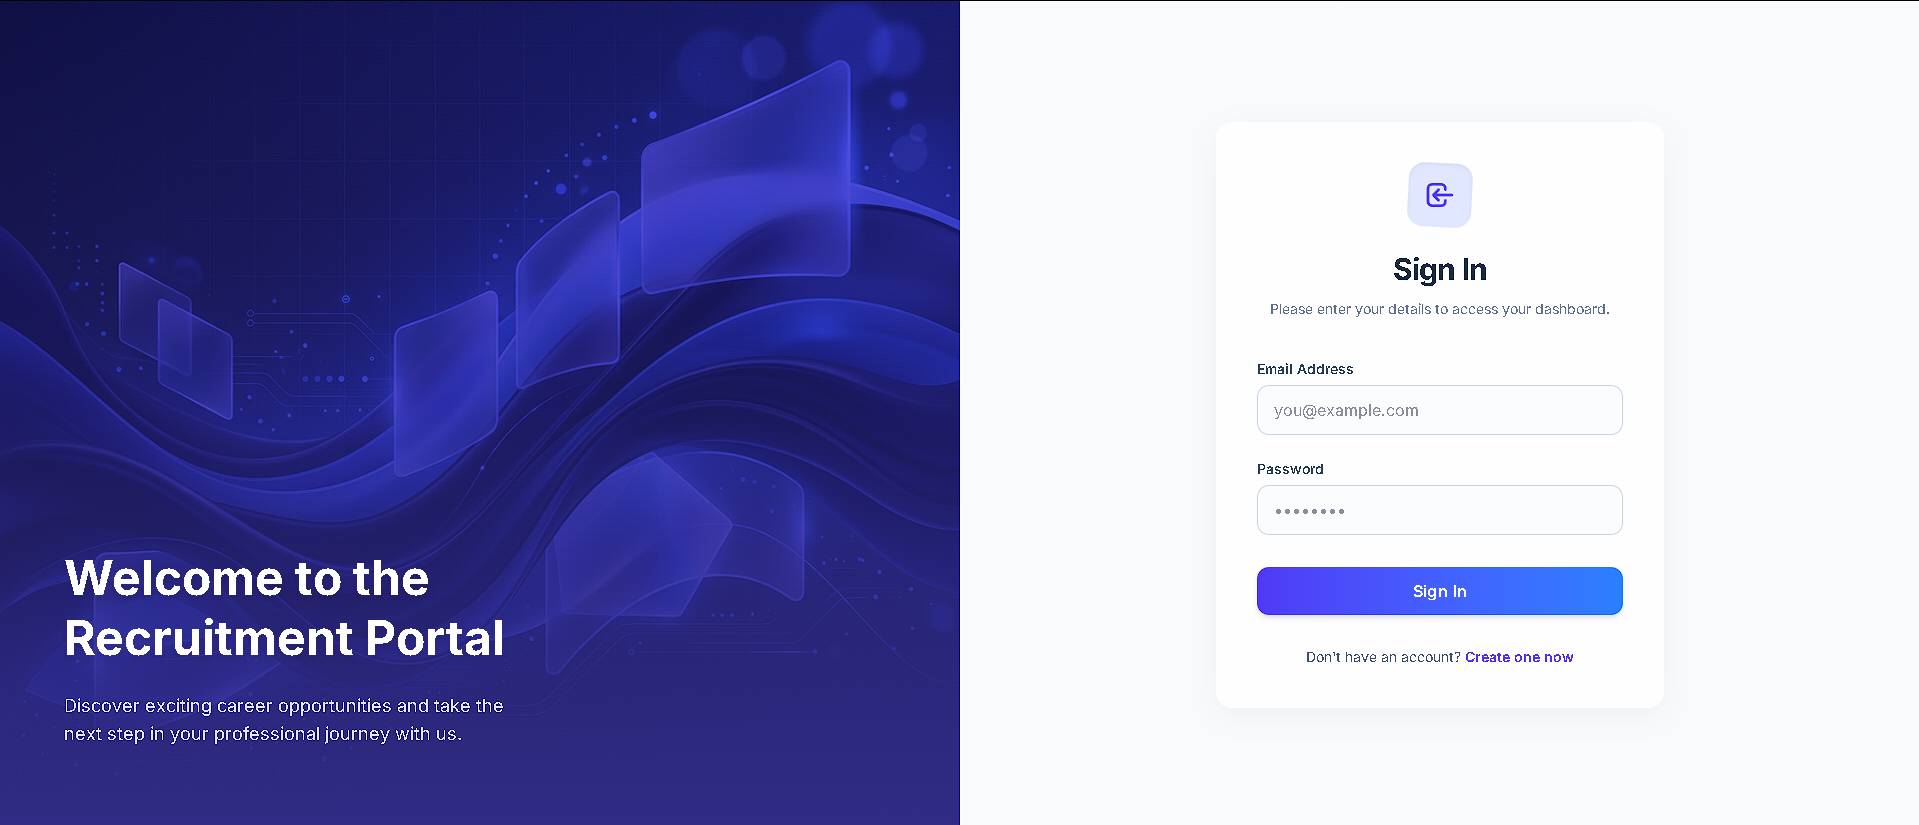
\includegraphics[width=\textwidth]{figures/student_login.png}}
    \caption{Student Login.}
  \end{minipage}\hfill
  \begin{minipage}{0.48\textwidth}
    \centering
    \fbox{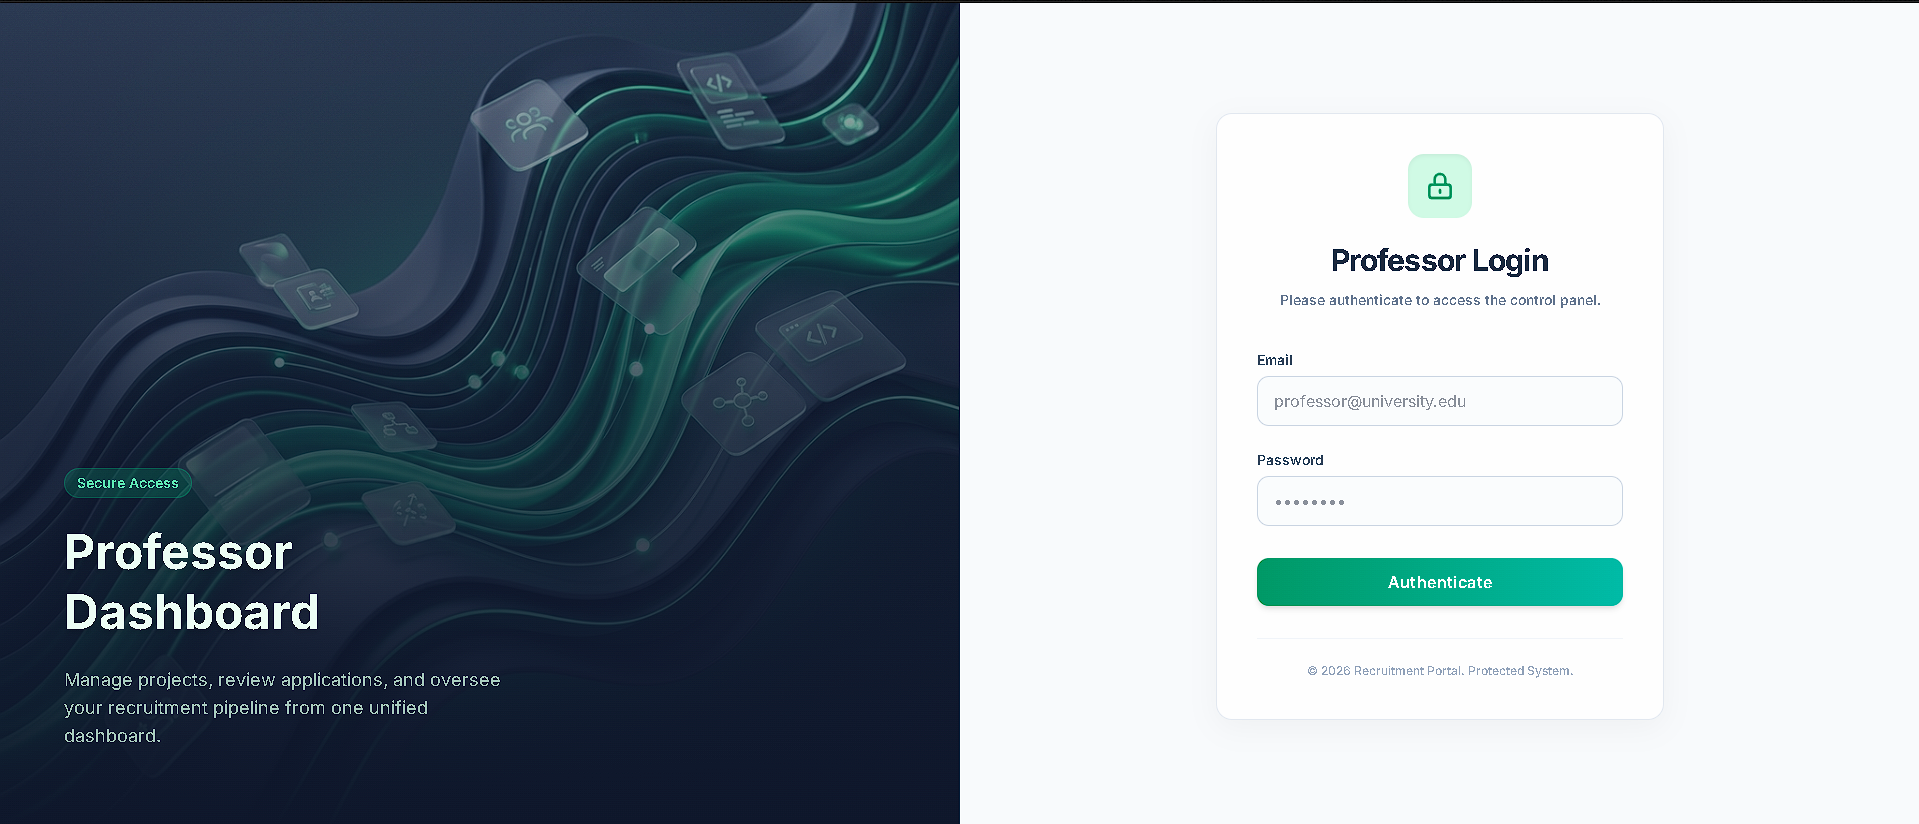
\includegraphics[width=\textwidth]{figures/professor_login.png}}
    \caption{Professor Login.}
  \end{minipage}
  
  \vspace{1ex}
  
  \begin{minipage}{0.48\textwidth}
    \centering
    \fbox{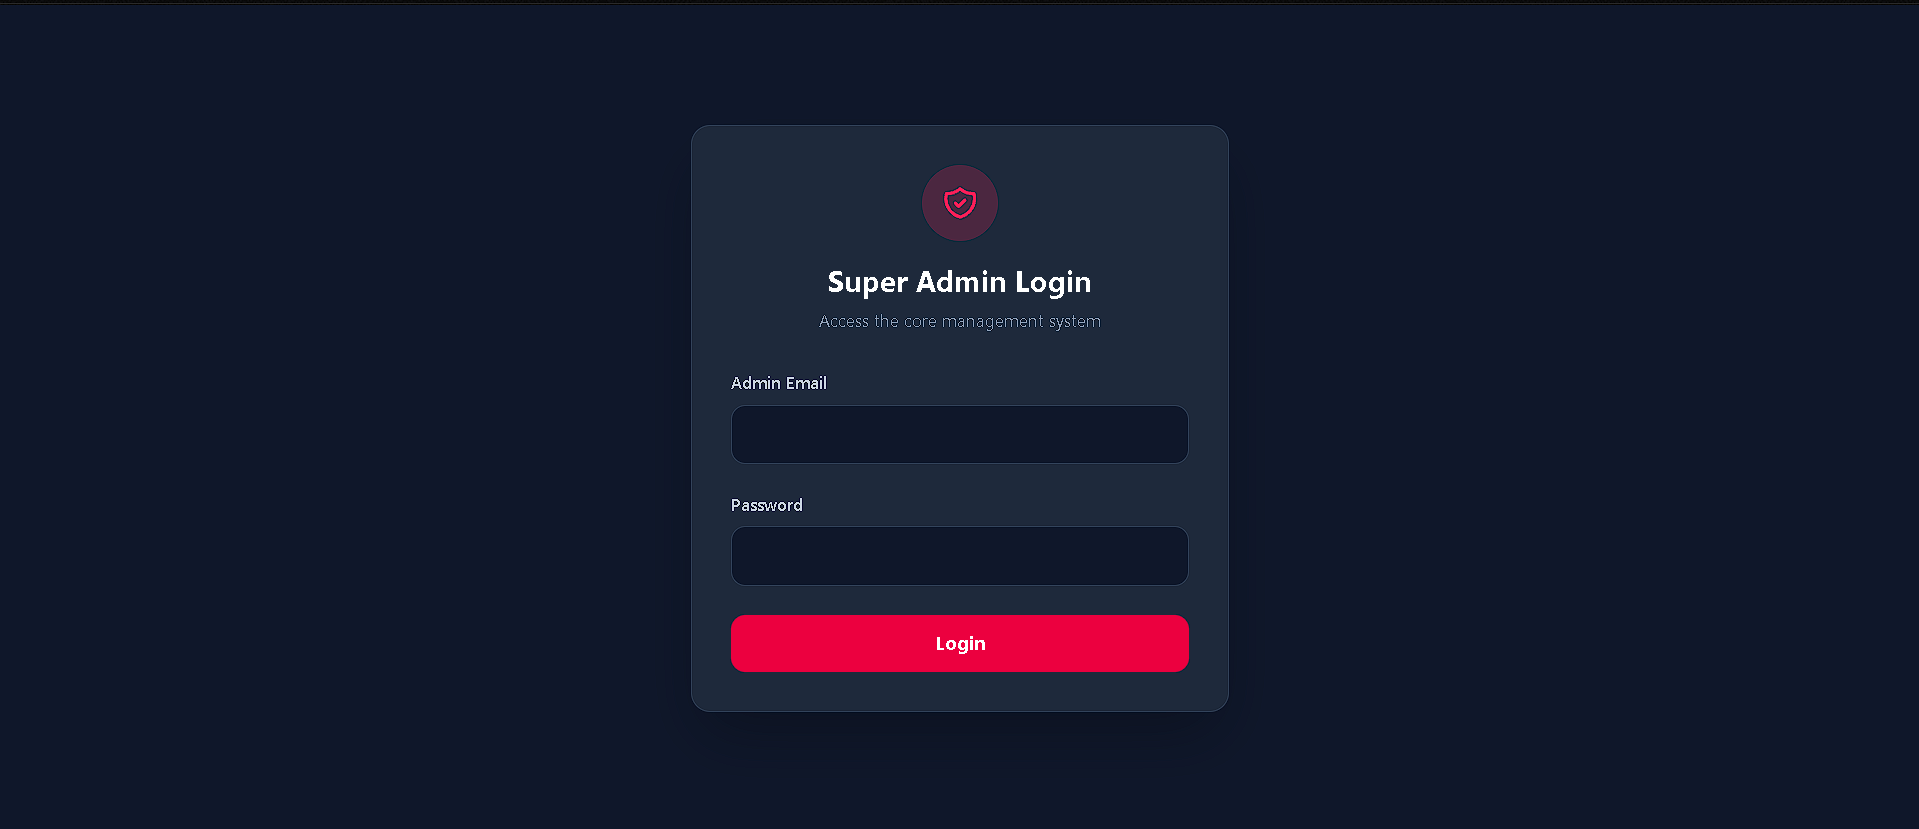
\includegraphics[width=\textwidth]{figures/admin_login.png}}
    \caption{Admin Login.}
  \end{minipage}
\end{figure}

\subsubsection{Professor Workflow}

Professors can create new project listings and manage applications received for their projects.

\begin{figure}[H]
  \centering
  \setlength{\fboxsep}{0pt}
  \setlength{\fboxrule}{0.2pt}
  \fbox{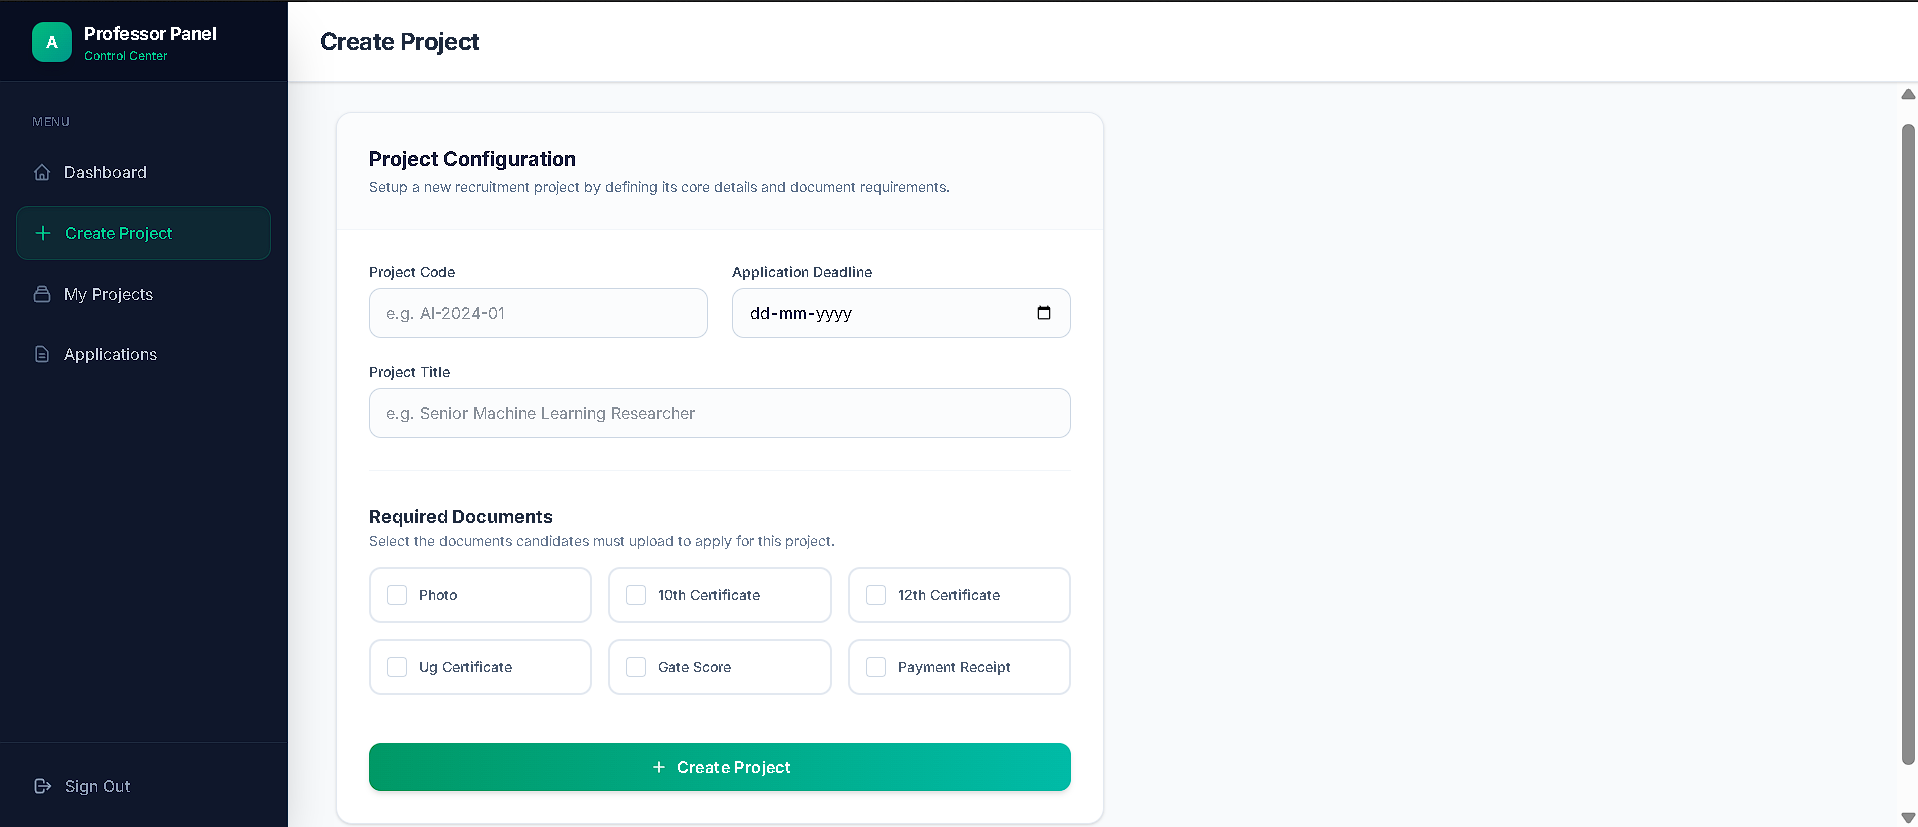
\includegraphics[width=0.85\textwidth]{figures/create_project.png}}
  \caption{Interface for creating a new project listing.}
  \label{fig:create_proj}
\end{figure}

\begin{figure}[H]
  \centering
  \setlength{\fboxsep}{0pt}
  \setlength{\fboxrule}{0.2pt}
  \fbox{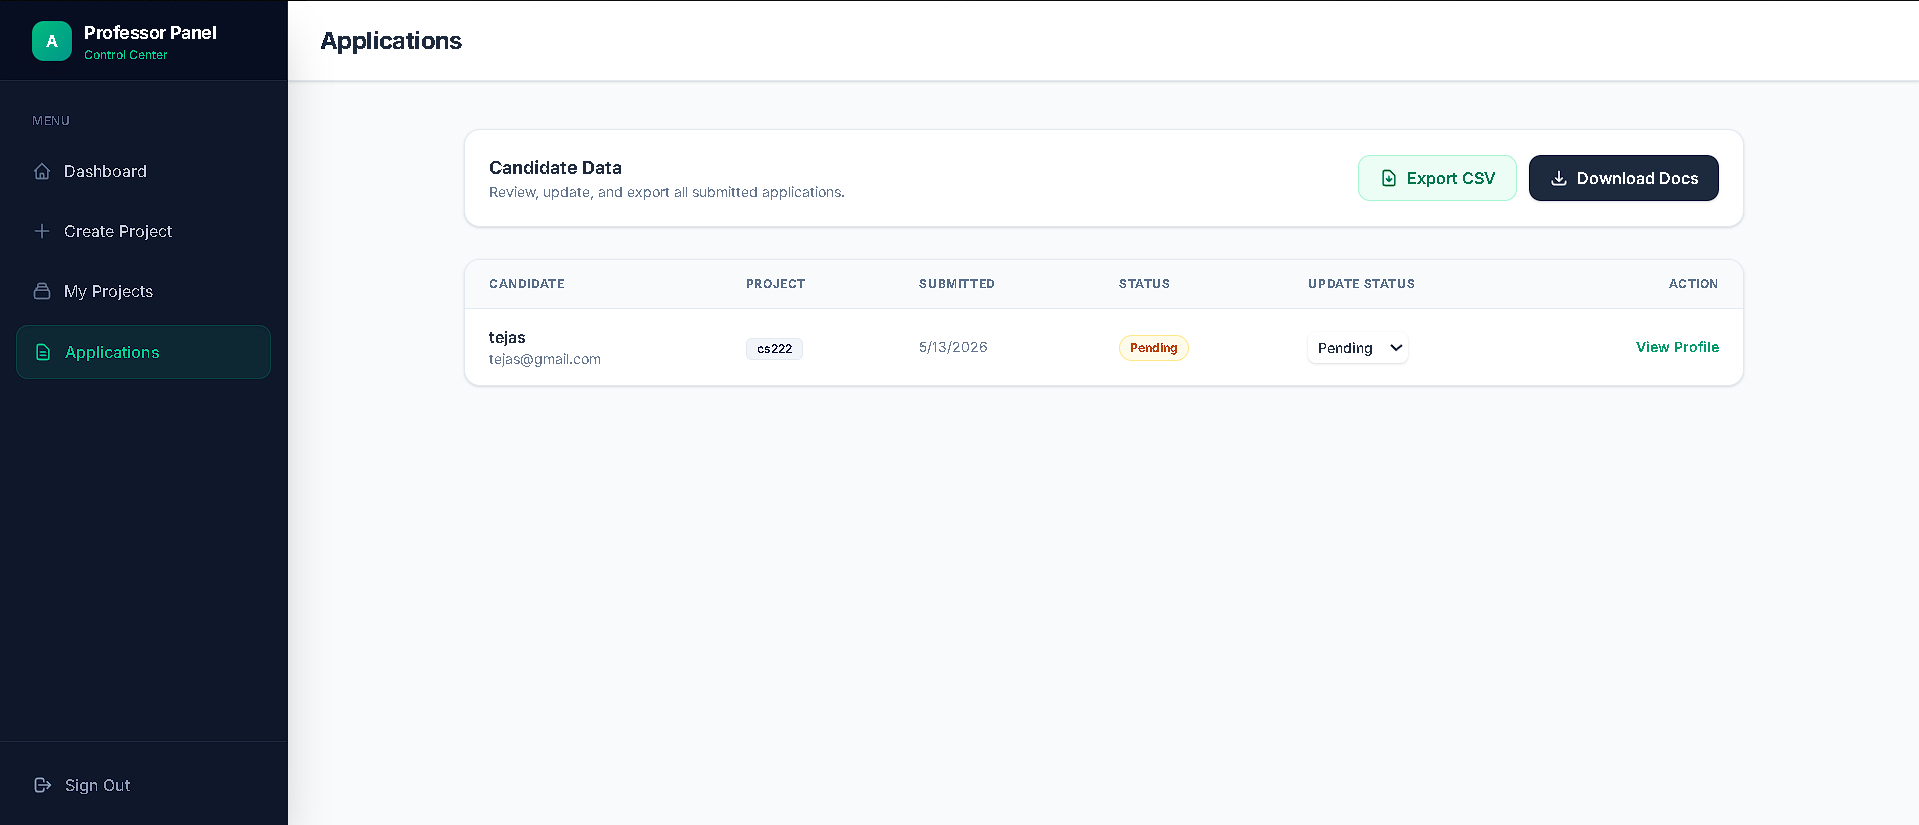
\includegraphics[width=0.85\textwidth]{figures/professor_studentapplications.png}}
  \caption{Professor's view of students who applied for a specific project.}
  \label{fig:prof_apps}
\end{figure}

\subsubsection{Administrative Management}

The Administrator has tools to moderate projects and view applications across the entire institution.

\begin{figure}[H]
  \centering
  \setlength{\fboxsep}{0pt}
  \setlength{\fboxrule}{0.2pt}
  \fbox{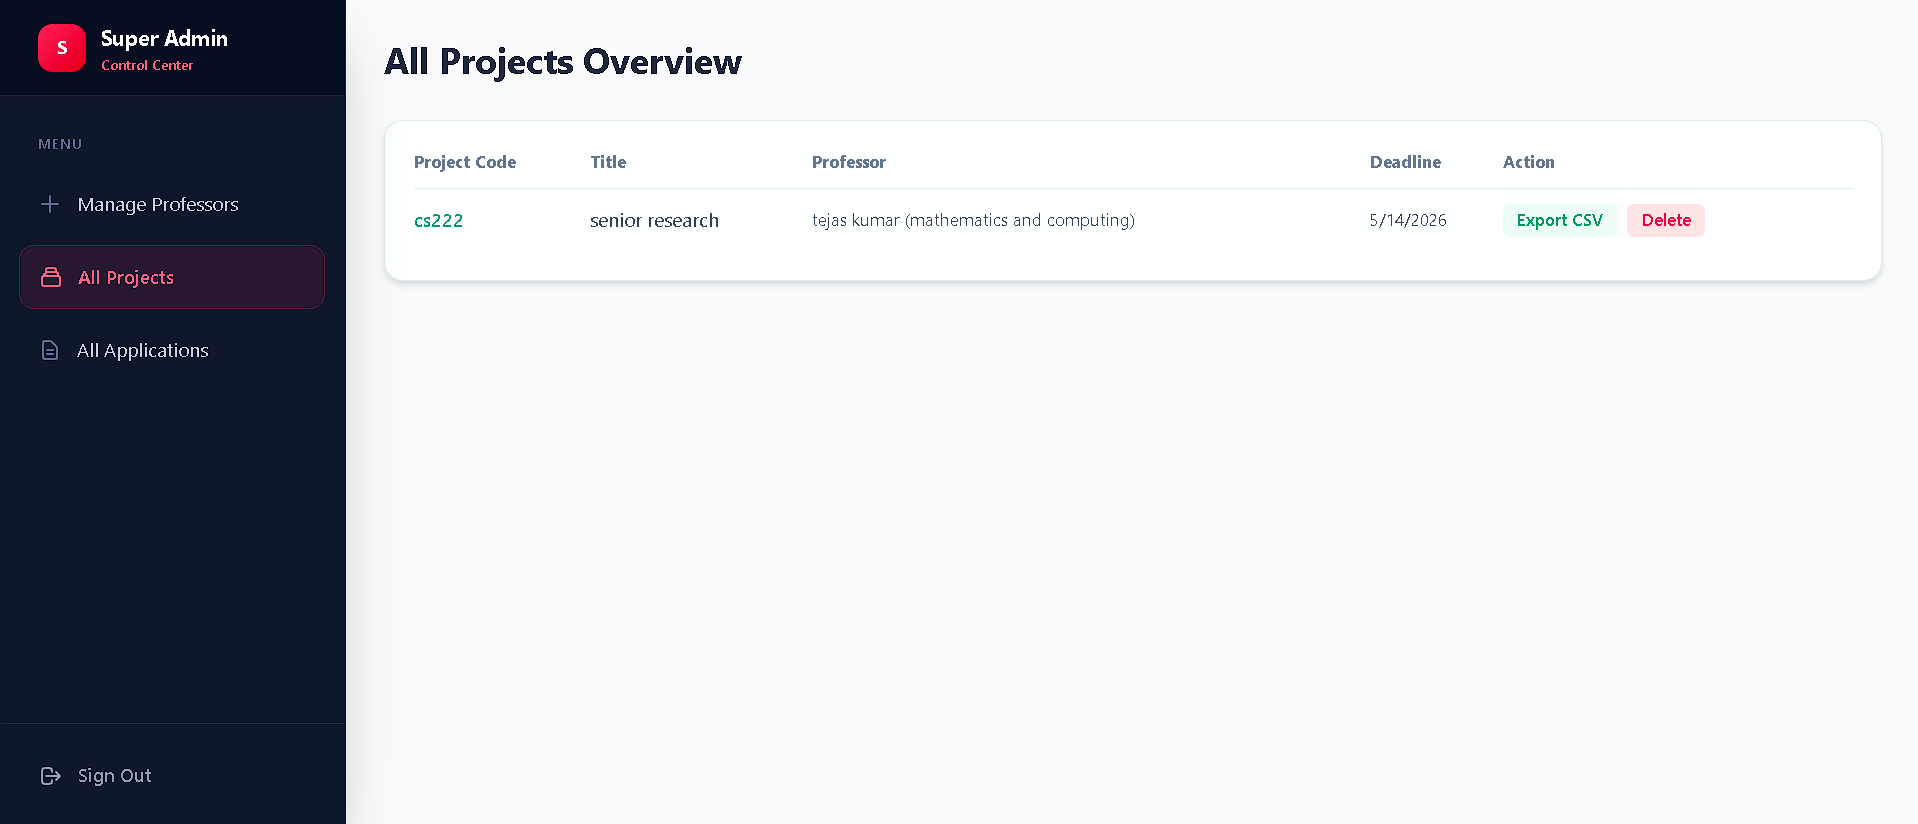
\includegraphics[width=0.85\textwidth]{figures/admin_allprojectoverview.png}}
  \caption{Admin overview of all projects currently listed on the portal.}
  \label{fig:admin_proj}
\end{figure}

\begin{figure}[H]
  \centering
  \setlength{\fboxsep}{0pt}
  \setlength{\fboxrule}{0.2pt}
  \fbox{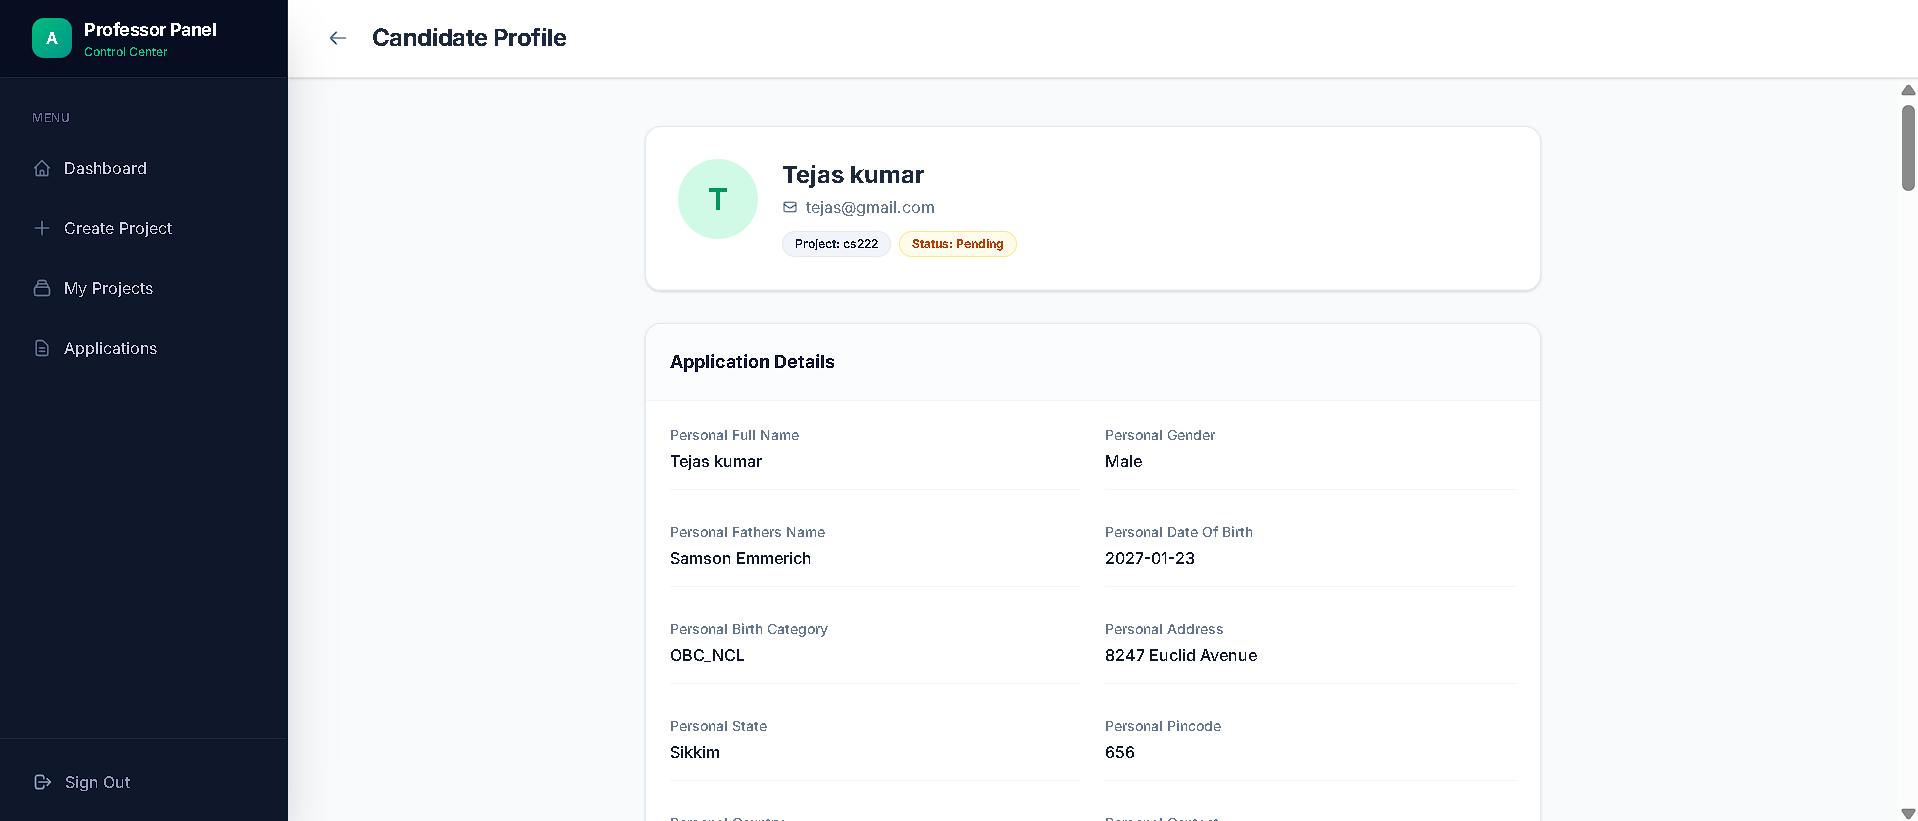
\includegraphics[width=0.85\textwidth]{figures/studentapplication_viewprofile.png}}
  \caption{Detailed view of an applicant's profile and submitted documents.}
  \label{fig:app_profile}
\end{figure}

\begin{figure}[H]
  \centering
  \setlength{\fboxsep}{0pt}
  \setlength{\fboxrule}{0.2pt}
  \fbox{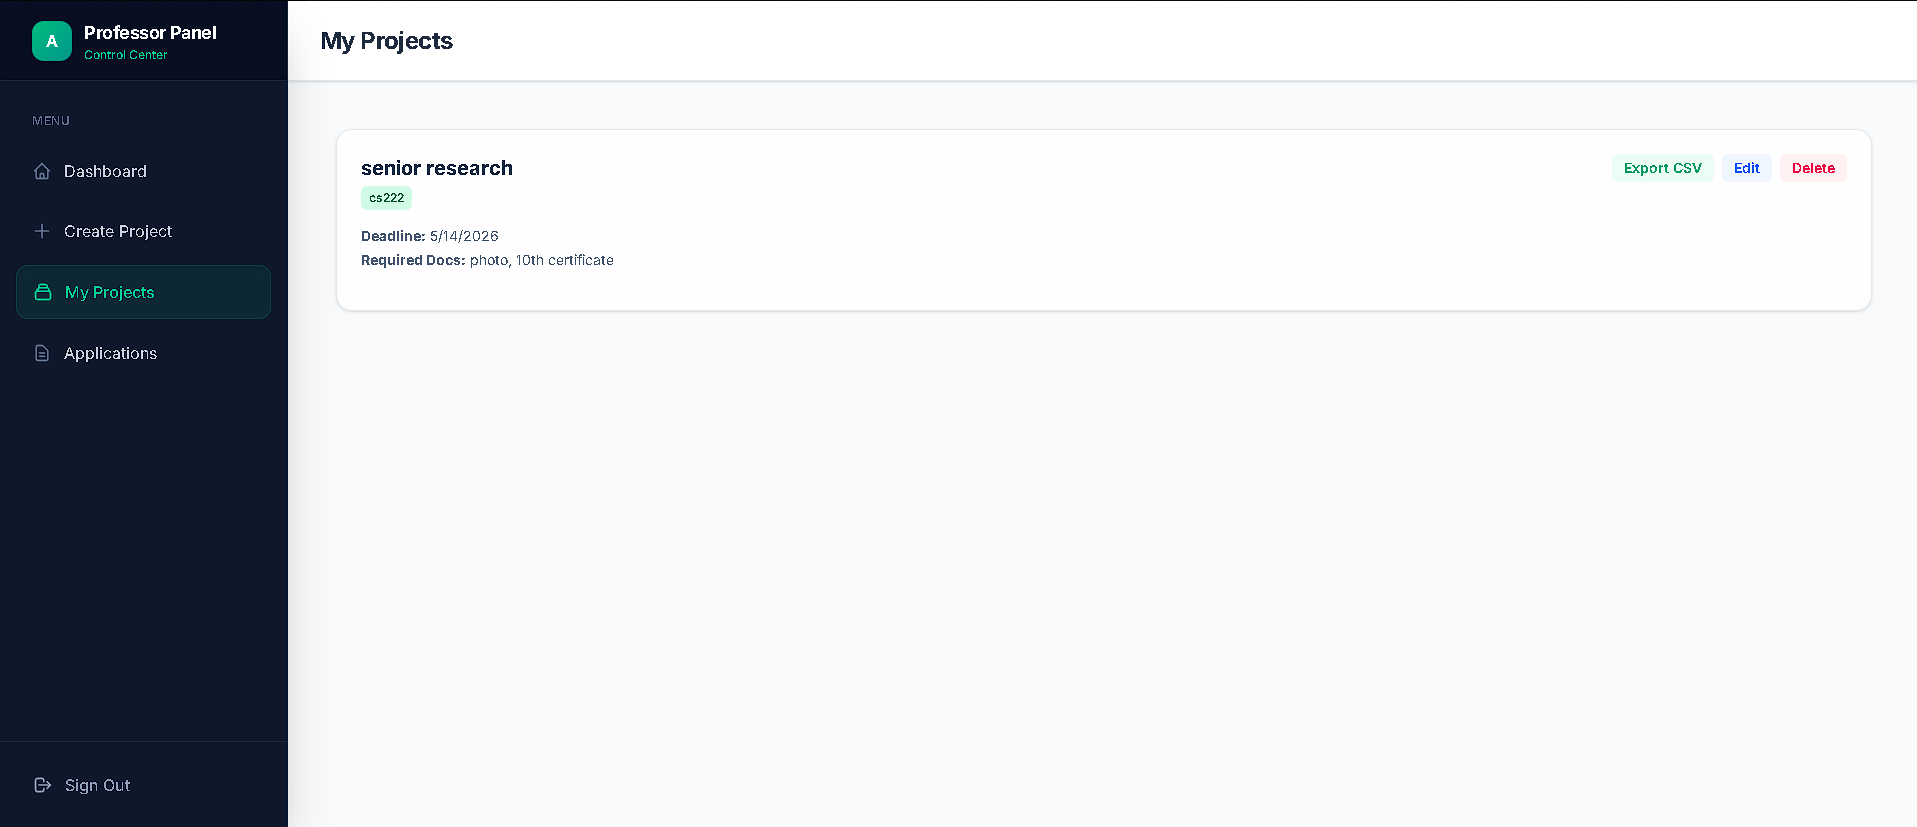
\includegraphics[width=0.85\textwidth]{figures/professor_myproject.png}}
  \caption{Professor's management view listing all projects created by them.}
  \label{fig:prof_projects}
\end{figure}

\begin{figure}[H]
  \centering
  \setlength{\fboxsep}{0pt}
  \setlength{\fboxrule}{0.2pt}
  \fbox{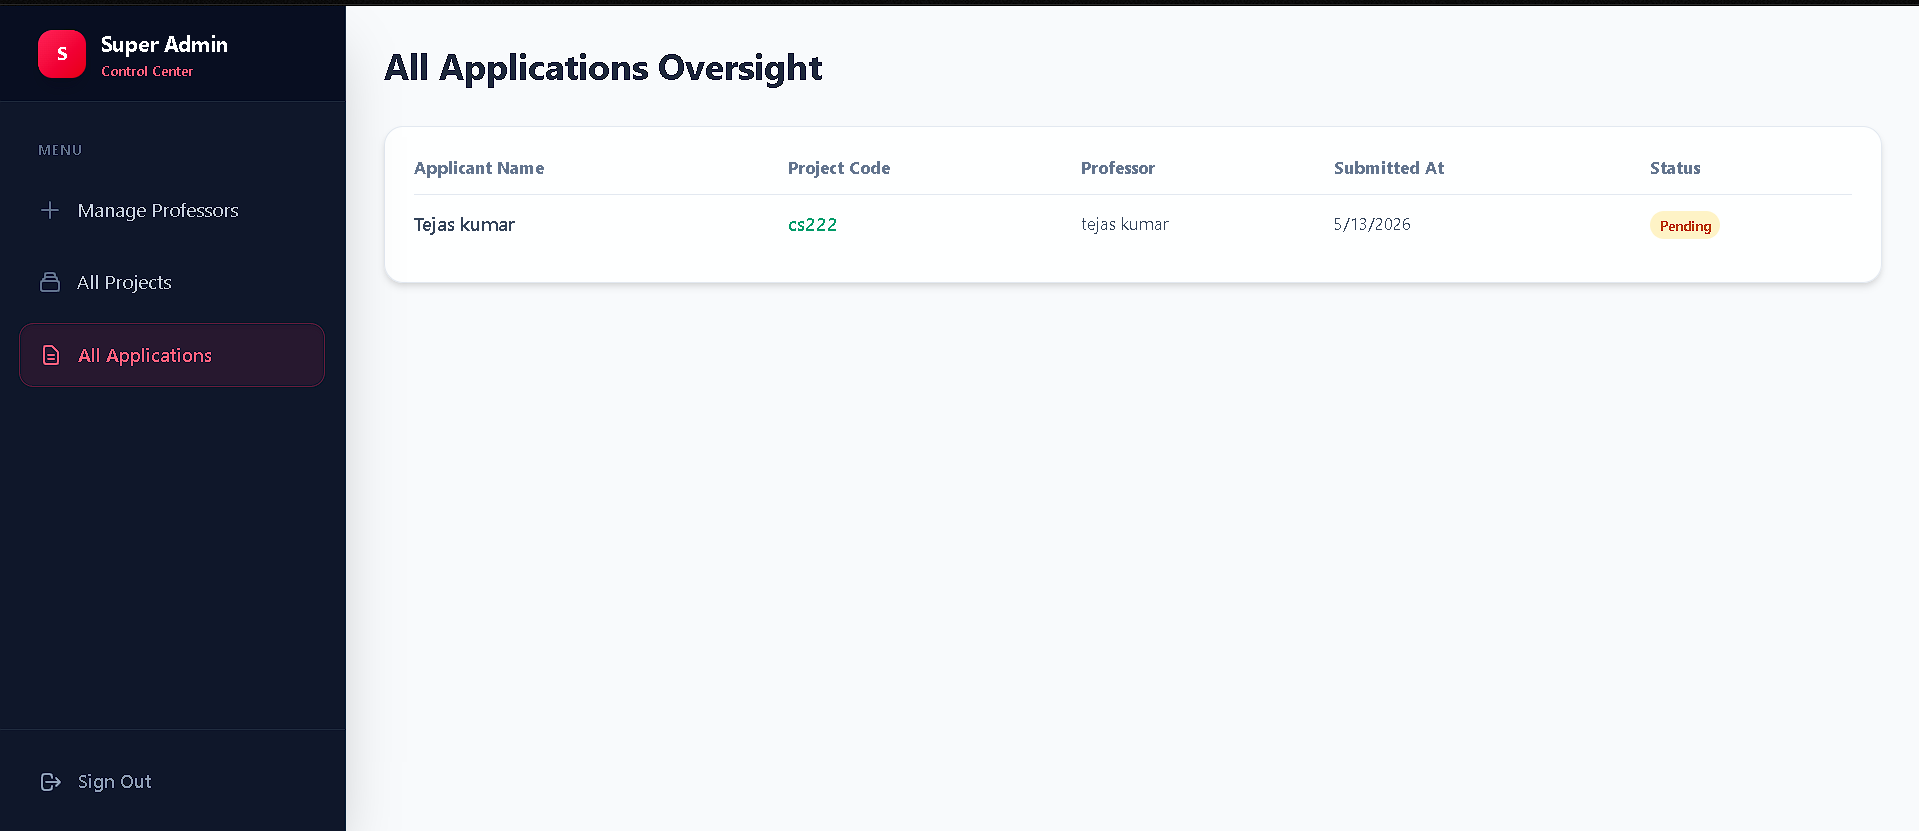
\includegraphics[width=0.85\textwidth]{figures/admin_allapplications.png}}
  \caption{Admin view showing all applications received across all institutional projects.}
  \label{fig:admin_apps}
\end{figure}

\section{Deployment and Containerization}

The system is containerized into three main services: `backend`, `frontend`, and `database`. Docker Compose manages the orchestration and networking between these services.

\begin{lstlisting}[language=bash, caption={Docker Compose service overview.}]
services:
  backend:
    build: ./backend
    volumes:
      - uploads_data:/app/uploads
  frontend:
    build: ./frontend
  db:
    image: mongo:latest
\end{lstlisting}

A named volume `uploads_data` is used to persist uploaded files outside the backend container's ephemeral storage.

\section{Security Implementation}

The system integrates several security hardening measures to protect sensitive applicant data. Table~\ref{tab:security} summarizes the key security features and the specific threats they mitigate.

\begin{table}[H]
  \centering
  \caption{Security features and threat mitigation in the Recruitment Portal.}
  \label{tab:security}
  \begin{tabularx}{\textwidth}{lX}
    \hline
    \textbf{Security Feature} & \textbf{Threat Mitigation} \\
    \hline
    Bcrypt Hashing (12 rounds) & Protects user passwords against brute-force and rainbow table attacks. \\
    JWT (Stateless Auth)       & Mitigates session fixation and CSRF risks by avoiding server-side session state. \\
    Express Validator          & Prevents NoSQL injection and XSS by sanitizing all incoming request bodies. \\
    Helmet.js Headers          & Enables CSP and HSTS to protect against cross-site scripting and protocol downgrades. \\
    Rate Limiting              & Protects the login and registration endpoints from automated dictionary attacks. \\
    \hline
  \end{tabularx}
\end{table}

\cleardoublepage
\typeout{}
% \chapter{Testing and Evaluation}

The current chapter analyzes MedTrack in terms of three aspects, namely, correctness (is the software implemented according to specifications?), security (can it withstand all possible types of attacks for which it is designed?), and performance (is it fast enough, does it respond within the required time limits for the typical load of a health center?).

\section{Testing Methodology}

Tests were carried out in a local Docker environment replicating the
environmental conditions expected during deployment - MongoDB in one
container, Express API server in another, and Nginx acting as the
web server for the React front end application hosted in the third.
The tests carried out were done against live data operations, as there
were no mock objects created - thereby guaranteeing true behavior
simulation during test execution.

Scenario-based testing was used for functional testing, where the test
scenario would cover the entire workflow of the user role from login
up to the completion of its last action. Adversarial input data were
used in security testing to simulate vulnerabilities targeted for
mitigation. Performance testing results were obtained using multiple API
requests, where their response times were measured on the server side.

\section{Functional Testing}

\subsection{Authentication Module}

\begin{itemize}
  \item A student signed in using the roll number \texttt{2201AI40}
  and the correct password. Expected: token issued, role-based dashboard
  displayed. \textbf{Result: Pass.}

  \item The same student entered an invalid password five consecutive
  times. Expected: account becomes locked on the fifth attempt,
  HTTP 403 status on the sixth attempt with the lockout message.
  \textbf{Result: Pass.}

  \item An account creation link was generated for a new account.
  The link was activated once successfully. Using the link again
  resulted in HTTP 400 status with the message "Token Already Consumed."
  \textbf{Result: Pass.}

  \item A student tried to access the doctor dashboard by directly
  visiting \texttt{/doctor/dashboard}. Expected: redirection to sign-in
  page due to Protected Route role verification. \textbf{Result: Pass.}
\end{itemize}

\subsection{Patient Management}

\begin{itemize}
  \item Another student registered and was assigned UHID \texttt{STU000001}.
  The subsequent student who registered got \texttt{STU000002}.
  Sequential UHID generation proved successful.
  \textbf{Result: Pass.}

  \item Another faculty registered a dependent (spouse). The spouse
  showed up in the admin’s pending verification list. Once approved,
  the spouse could be searched by the staff for consultation booking.
  Prior to being approved, searching the spouse by the staff produced
  no results. \textbf{Result: Pass.}

  \item An administrator soft-deleted a patient record. The patient
  vanished from all list screens. Then, the administrator restored
  the patient using the accordion menu for deleted records. The
  patient reappeared with all past consultations intact. \textbf{Result:
    Pass.}

  \item A patient uploaded a profile picture that was greater than
  5\,MB in size. The system refused the upload without saving the
  file. \textbf{Result: Pass.}
\end{itemize}

\subsection{Consultation Workflow}

\begin{itemize}
  \item Staff Member created a consultation for the student \texttt{2201AI40}. A consultation was assigned to the doctor. The pending queue of the doctor was updated instantly upon reloading the next page. An in-app notification appeared under the doctor’s notification bell. \textbf{Result: Pass.}

  \item The doctor accessed the consultation. The consultations conducted by the patient before and the uploaded lab reports were seen in the left side panel. The doctor filled out the prescription and submitted it. The consultation was marked as complete and the patient got an in-app notification. \textbf{Result: Pass.}

  \item A Staff Member assigned an incomplete consultation to Doctor A to Doctor B. The consultation could not be seen in the queue of Doctor A while it was available in the queue of Doctor B. The notifications of both doctors were updated instantly. \textbf{Result: Pass.}

  \item A doctor flagged the consultation for follow-up in 7 days. The follow-up date was printed in the generated PDF. \textbf{Result: Pass.}
\end{itemize}

\subsection{PDF Prescription Generation}

\begin{itemize}
  \item Prescription was created with two medications and a lab test.
  The PDF had all required details: Header with name of IIT Patna
  Health Centre, patient details including name, UHID, blood group,
  roll number, any allergic history, clinical notes, medicine
  table, and finally, the name of the doctor. \textbf{Result: Pass}

  \item A user tried to view another person’s prescription PDF by
  making a guess for the URL without providing any valid JSON web
  token. HTTP 401 response was received because there was no
  authentication done. \textbf{Result: Pass}
\end{itemize}

\subsection{Laboratory Report Management}

\begin{itemize}
  \item A lab report in PDF format was uploaded by a patient. The
  report showed up on the Reports page for that patient and could be
  seen by the doctor on the patient history screen within the new
  consultation process. \textbf{Result: Pass.}

  \item One of a patient’s reports was deleted. The document was
  deleted both on disk and in the database. This report no longer
  showed up in the list for that patient or the doctor’s history
  screen. \textbf{Result: Pass.}
\end{itemize}

\subsection{Notification System}

\begin{itemize}
  \item All four trigger events (consultation created, consultation
  completed, dependent registration, dependent verification) were
  performed. In all cases, the right person was notified and the
  bell badge number was increased. \textbf{Result: Pass.}

  \item Reading notifications lowered the number of badges by one.
  Reading all lowered the number of badges to zero.
  \textbf{Result: Pass.}
\end{itemize}

\subsection{Administrative Analytics}

\begin{itemize}
  \item Following the seeding of 30 consultations within 7 days, the trend graph showed the correct number of consultations per day. The summary number of the last seven days tallied with the total number in the graph. \textbf{Result: Passed}

  \item The physician productivity table ranked physicians correctly according to their number of consultations, having taken into account consultations from more than one physician. \textbf{Result: Passed}
\end{itemize}

Table~\ref{tab:features} summarises the objective-to-feature validation
matrix for all stated project objectives.

\begin{table}[htbp]
  \centering
  \caption{Objective-to-feature validation matrix.}
  \label{tab:features}
  \begin{tabularx}{\textwidth}{lXl}
    \hline
    \textbf{Obj.} & \textbf{Implemented Feature} & \textbf{Result} \\
    \hline
    O1 & Centralised patient repository: profile, medical info,
         document storage, soft delete
       & Pass \\
    O2 & Queue-based consultation workflow: Staff creates, Doctor
         completes, real-time status update
       & Pass \\
    O3 & Structured prescription form and automated PDF generation
         with IIT Patna Health Centre header
       & Pass \\
    O4 & Authenticated lab report upload, inline view, and delete
       & Pass \\
    O5 & Faculty-dependent registration with admin approval workflow
       & Pass \\
    O6 & JWT + RBAC enforced on every protected endpoint; four
         distinct role access sets
       & Pass \\
    O7 & bcrypt, rate limiting, Helmet, input validation, ReDoS
         prevention, mass-assignment protection
       & Pass \\
    O8 & Admin analytics: daily/monthly charts, demographics, doctor
         productivity, inventory summary
       & Pass \\
    O9 & In-app notification bell with four trigger events
       & Pass \\
    \hline
  \end{tabularx}
\end{table}

\section{Security Testing}

The security posture of MedTrack was compared with the
OWASP Top Ten Risk Categories for the year 2021 \cite{OWASP2021}
that are applicable to a web-based healthcare application.
Table~\ref{tab:owasp} describes each of these risks, the

\begin{table}[htbp]
  \centering
  \caption{OWASP Top Ten 2021 mitigation and test results.}
  \label{tab:owasp}
  \begin{tabularx}{\textwidth}{lXl}
    \hline
    \textbf{Risk} & \textbf{Mitigation in MedTrack} & \textbf{Result} \\
    \hline
    A01: Broken Access Control
      & JWT + RBAC; ownership checks on file ops and dependent
        registration
      & Pass \\
    A02: Cryptographic Failures
      & bcryptjs (cost 10) for passwords; JWT over TLS; no plaintext
        credential storage
      & Pass \\
    A03: Injection
      & express-validator on all inputs; \texttt{escapeRegex} on
        search; Mongoose parameterised queries
      & Pass \\
    A04: Insecure Design
      & Threat-modelled auth flow; soft delete; append-only audit
        log; single-use password tokens
      & Pass \\
    A05: Security Misconfiguration
      & Helmet HTTP headers; CORS whitelist; env variable validation
        on startup
      & Pass \\
    A07: Identification and Auth Failures
      & Account lockout after 5 attempts; rate limiting on login;
        24-hour JWT expiry
      & Pass \\
    A09: Security Logging Failures
      & Winston structured logs; AuditLog for all sensitive ops
        with actor, IP, timestamp
      & Pass \\
    \hline
  \end{tabularx}
\end{table}

\subsection{Privilege Escalation Test (Mass-Assignment)}

A PATCH request was made to the endpoint that updates the patient profile with the extra attribute \texttt{"role": "admin"}. The field whitelist of the update controller did not consider the \texttt{role} field at all. A check on the database entry confirmed that the user’s role had not been changed at all. \textbf{Outcome: Pass.}

\subsection{ReDoS Resistance Test}

A search string that causes catastrophic backtracking due to
a naive regex such as a repeated pattern followed by a non-matching
character was sent to the patient search endpoint. The string was
sanitized with the \texttt{escapeRegex()} function before sending,
and all special characters were escaped in the string before it was
passed into the query. The request was completed instantaneously and
returned an empty array of results. \textbf{Result: Pass.}

\subsection{Brute-Force Resistance Test}

Six successive login attempts using invalid credentials were made on the same user account. The results of the first five were HTTP 401 (invalid credentials). The sixth resulted in HTTP 403 with a message ``Account locked. Please try after 15 minutes,'' indicating that lockout and cooldown are functioning properly. \textbf{Conclusion: Pass.}

\subsection{Unauthorised File Access Test}

\begin{sloppypar}
The request to the prescription file API endpoint \texttt{/api/consultations/:id/pdf} using the \texttt{GET} method was made without an \texttt{Authorization} header, which resulted in an HTTP 401 response. Another request was made using a valid JWT but for a different user, and an HTTP 403 response was received. This proves that the ownership validation rule is implemented, i.e., only the patient, his doctor, or an administrator can access the file. \textbf{Conclusion: Passed.}
\end{sloppypar}

\subsection{JWT Expiry Test}

\begin{sloppypar}
An expired JWT (manually constructed with a past \texttt{exp} claim)
was submitted to a protected endpoint. The \texttt{protect} middleware
caught the \texttt{TokenExpiredError} from \texttt{jwt.verify()} and
returned HTTP 401. The frontend's Axios interceptor detected the 401
and displayed the \texttt{SessionExpiredBanner}. \textbf{Result: Pass.}
\end{sloppypar}

\section{Performance Testing}

Performance was measured on a development machine (Intel Core i7,
16\,GB RAM) running all three Docker containers. Each endpoint was
called 10 times in succession; the values in Table~\ref{tab:perf}
represent the average response time.

\begin{table}[htbp]
  \centering
  \caption{Average API response times under single-user load.}
  \label{tab:perf}
  \begin{tabular}{lrl}
    \hline
    \textbf{Endpoint} & \textbf{Avg.\ (ms)} & \textbf{Bottleneck} \\
    \hline
    POST /api/auth/login              & 185 & bcrypt.compare() \\
    GET  /api/patients (page 1)       &  42 & Indexed query \\
    POST /api/consultations           &  58 & DB write + notification \\
    PUT  /api/consultations/:id (complete) & 510 & PDF generation (sync) \\
    GET  /api/dashboard               &  92 & Aggregation pipeline \\
    GET  /api/audit                   &  48 & Paginated index scan \\
    GET  /api/notifications           &  35 & Simple filter query \\
    POST /api/reports (file upload)   & 120 & Disk write \\
    \hline
  \end{tabular}
\end{table}

Apart from consultation completion, all endpoints complete in less
than 200\,ms, which is unnoticeable for users. The delay of
510\,ms in consultation completion is due to synchronous PDF
generation during HTTP response processing. This is fine, considering
the anticipated number of concurrent users (up to several tens) at a
large institutional health centre. For more significant numbers, the
suggestion is to asynchronously generate PDFs using a background job
queue as a potential enhancement.

\subsection{Scalability Issue Identified}

The \texttt{GET /api/patients} endpoint currently queries all
records of Student and Faculty types from the \texttt{User}
collection and all Dependent records from the \texttt{Patient}
collection. All queried records are loaded into Node.js heap memory,
merged and sorted on JavaScript, and sliced according to the desired
page. While this works perfectly well for IIT Patna's population,
it is likely to cause out-of-memory issues for a larger institution.
The recommended solution -- merging and paginating all records using
a single MongoDB aggregation pipeline -- is noted as future work.

\section{Comparison with Existing Systems}

Table~\ref{tab:comparison} compares MedTrack with OpenMRS~\cite{OpenMRS2006},
a widely used open-source EMR for resource-limited settings, and with a
representative generic MERN-based HIS prototype typical of academic
implementations.

\begin{table}[htbp]
  \centering
  \caption{Feature comparison: MedTrack vs.\ existing systems.}
  \label{tab:comparison}
  \begin{tabularx}{\textwidth}{Xccc}
    \hline
    \textbf{Feature} & \textbf{MedTrack} & \textbf{OpenMRS}
                     & \textbf{Generic MERN HIS} \\
    \hline
    Lightweight single-institution setup  & Yes & No  & Yes \\
    Institutional ID-based auth           & Yes & No  & No  \\
    Faculty-dependent patient hierarchy   & Yes & No  & No  \\
    Automated PDF prescription            & Yes & No  & No  \\
    Soft delete with restore              & Yes & No  & No  \\
    Append-only audit log                 & Yes & Yes & No  \\
    In-app notification system            & Yes & No  & No  \\
    Role-based access control (4 roles)   & Yes & Yes & Partial \\
    Rate limiting on login                & Yes & No  & No  \\
    ReDoS-safe search                     & Yes & N/A & No  \\
    Mass-assignment protection            & Yes & N/A & No  \\
    Docker containerisation               & Yes & No  & Partial \\
    Admin analytics with charts           & Yes & No  & No  \\
    Doctor prescription shortcuts         & Yes & No  & No  \\
    \hline
  \end{tabularx}
\end{table}

MedTrack offers more comprehensive and more robust features compared to the two competing options. Compared to OpenMRS, MedTrack demands significantly fewer setup and deployment efforts. Compared to a generic prototype developed using the MERN stack, it comes with the additional benefits of security enhancements, compliance capabilities, and the unique identity model of IIT Patna.

% \cleardoublepage
% \typeout{}
\chapter{Conclusion and Future Work}

\section{Conclusion}

The Institutional Recruitment Portal has been developed to digitize and streamline the recruitment process for academic projects. By replacing manual, email-based workflows with a secure MERN-stack platform, the system significantly improves organizational efficiency for both professors and administrative staff.

The system features a robust, role-based architecture that caters to Applicants, Professors, and Administrators. Key technical achievements include the implementation of a structured local file storage system, bulk data export capabilities (ZIP and CSV), and a secure authentication framework. The use of Docker ensures that the system is easily deployable and scalable within an institutional IT environment.

Evaluation of the portal shows that it effectively addresses the primary challenges of application fragmentation and manual document management. It provides a professional and transparent interface for applicants while giving professors the tools they need to manage recruitment at scale.

\section{Limitations}

Despite its functionality, the current version has some limitations:

\begin{enumerate}
  \item \textbf{Manual Approval for Professors:} Currently, professors must be manually approved by an admin, which can cause delays during peak recruitment periods.
  
  \item \textbf{Basic Search Functionality:} The project search is based on simple keyword matching and could be improved with more advanced filtering.
  
  \item \textbf{Lack of Real-time Notifications:} The system does not currently notify users of status changes via email or SMS in real-time.
  
  \item \textbf{No Automated Screening:} Professors still need to manually review every application; there is no automated ranking or screening based on qualifications.
\end{enumerate}

\section{Future Work}

Several areas have been identified for future enhancement:

\begin{itemize}
  \item \textbf{AI-Based Applicant Ranking:} Integrating a machine learning module to rank applicants based on their skills and credentials relative to project requirements.
  
  \item \textbf{Email and SMS Integration:} Adding automated email notifications for application submission confirmations and status updates.
  
  \item \textbf{Integrated Interview Module:} Developing a built-in scheduling and video conferencing tool for conducting online interviews within the portal.
  
  \item \textbf{Advanced Analytics:} Implementing a more detailed analytics dashboard for admins to track recruitment trends and diversity metrics.
  
  \item \textbf{Public API:} Developing a documented REST API to allow integration with other institutional ERP systems.
\end{itemize}

In conclusion, the Institutional Recruitment Portal establishes a solid digital foundation for project-based hiring. It is a production-ready solution that can be further expanded to become a comprehensive human resource management tool for academic institutions.
\typeout{}

\bibliography{btp}
\bibliographystyle{ieeetr}
\end{document}
